\documentclass[twoside]{book}

% Packages required by doxygen
\usepackage{calc}
\usepackage{doxygen}
\usepackage{graphicx}
\usepackage[utf8]{inputenc}
\usepackage{makeidx}
\usepackage{multicol}
\usepackage{multirow}
\usepackage{textcomp}
\usepackage[table]{xcolor}

% Font selection
\usepackage[T1]{fontenc}
\usepackage{mathptmx}
\usepackage[scaled=.90]{helvet}
\usepackage{courier}
\usepackage{amssymb}
\usepackage{sectsty}
\renewcommand{\familydefault}{\sfdefault}
\allsectionsfont{%
  \fontseries{bc}\selectfont%
  \color{darkgray}%
}
\renewcommand{\DoxyLabelFont}{%
  \fontseries{bc}\selectfont%
  \color{darkgray}%
}

% Page & text layout
\usepackage{geometry}
\geometry{%
  a4paper,%
  top=2.5cm,%
  bottom=2.5cm,%
  left=2.5cm,%
  right=2.5cm%
}
\tolerance=750
\hfuzz=15pt
\hbadness=750
\setlength{\emergencystretch}{15pt}
\setlength{\parindent}{0cm}
\setlength{\parskip}{0.2cm}
\makeatletter
\renewcommand{\paragraph}{%
  \@startsection{paragraph}{4}{0ex}{-1.0ex}{1.0ex}{%
    \normalfont\normalsize\bfseries\SS@parafont%
  }%
}
\renewcommand{\subparagraph}{%
  \@startsection{subparagraph}{5}{0ex}{-1.0ex}{1.0ex}{%
    \normalfont\normalsize\bfseries\SS@subparafont%
  }%
}
\makeatother

% Headers & footers
\usepackage{fancyhdr}
\pagestyle{fancyplain}
\fancyhead[LE]{\fancyplain{}{\bfseries\thepage}}
\fancyhead[CE]{\fancyplain{}{}}
\fancyhead[RE]{\fancyplain{}{\bfseries\leftmark}}
\fancyhead[LO]{\fancyplain{}{\bfseries\rightmark}}
\fancyhead[CO]{\fancyplain{}{}}
\fancyhead[RO]{\fancyplain{}{\bfseries\thepage}}
\fancyfoot[LE]{\fancyplain{}{}}
\fancyfoot[CE]{\fancyplain{}{}}
\fancyfoot[RE]{\fancyplain{}{\bfseries\scriptsize Generated on Sun Mar 1 2015 18\-:31\-:49 for Arp\-Poisonning by Doxygen }}
\fancyfoot[LO]{\fancyplain{}{\bfseries\scriptsize Generated on Sun Mar 1 2015 18\-:31\-:49 for Arp\-Poisonning by Doxygen }}
\fancyfoot[CO]{\fancyplain{}{}}
\fancyfoot[RO]{\fancyplain{}{}}
\renewcommand{\footrulewidth}{0.4pt}
\renewcommand{\chaptermark}[1]{%
  \markboth{#1}{}%
}
\renewcommand{\sectionmark}[1]{%
  \markright{\thesection\ #1}%
}

% Indices & bibliography
\usepackage{natbib}
\usepackage[titles]{tocloft}
\setcounter{tocdepth}{3}
\setcounter{secnumdepth}{5}
\makeindex

% Hyperlinks (required, but should be loaded last)
\usepackage{ifpdf}
\ifpdf
  \usepackage[pdftex,pagebackref=true]{hyperref}
\else
  \usepackage[ps2pdf,pagebackref=true]{hyperref}
\fi
\hypersetup{%
  colorlinks=true,%
  linkcolor=blue,%
  citecolor=blue,%
  unicode%
}

% Custom commands
\newcommand{\clearemptydoublepage}{%
  \newpage{\pagestyle{empty}\cleardoublepage}%
}


%===== C O N T E N T S =====

\begin{document}

% Titlepage & ToC
\hypersetup{pageanchor=false}
\pagenumbering{roman}
\begin{titlepage}
\vspace*{7cm}
\begin{center}%
{\Large Arp\-Poisonning }\\
\vspace*{1cm}
{\large Generated by Doxygen 1.8.6}\\
\vspace*{0.5cm}
{\small Sun Mar 1 2015 18:31:49}\\
\end{center}
\end{titlepage}
\clearemptydoublepage
\tableofcontents
\clearemptydoublepage
\pagenumbering{arabic}
\hypersetup{pageanchor=true}

%--- Begin generated contents ---
\chapter{Hierarchical Index}
\section{Class Hierarchy}
This inheritance list is sorted roughly, but not completely, alphabetically\-:\begin{DoxyCompactList}
\item \contentsline{section}{Arp\-Spoofing}{\pageref{class_arp_spoofing}}{}
\item \contentsline{section}{Network\-Utilities}{\pageref{class_network_utilities}}{}
\item \contentsline{section}{Packet}{\pageref{class_packet}}{}
\begin{DoxyCompactList}
\item \contentsline{section}{Ethernet}{\pageref{class_ethernet}}{}
\begin{DoxyCompactList}
\item \contentsline{section}{Arp}{\pageref{class_arp}}{}
\end{DoxyCompactList}
\end{DoxyCompactList}
\item \contentsline{section}{uchar\-Mac}{\pageref{structuchar_mac}}{}
\item \contentsline{section}{uint8\-Ip}{\pageref{structuint8_ip}}{}
\end{DoxyCompactList}

\chapter{Class Index}
\section{Class List}
Here are the classes, structs, unions and interfaces with brief descriptions\-:\begin{DoxyCompactList}
\item\contentsline{section}{\hyperlink{class_arp}{Arp} \\*Class header for build A\-R\-P packet }{\pageref{class_arp}}{}
\item\contentsline{section}{\hyperlink{class_arp_spoofing}{Arp\-Spoofing} \\*Class header for run M\-I\-T\-M attack }{\pageref{class_arp_spoofing}}{}
\item\contentsline{section}{\hyperlink{class_ethernet}{Ethernet} \\*Class header for build \hyperlink{class_ethernet}{Ethernet} packet }{\pageref{class_ethernet}}{}
\item\contentsline{section}{\hyperlink{class_network_utilities}{Network\-Utilities} \\*Utilities class for implement network functions }{\pageref{class_network_utilities}}{}
\item\contentsline{section}{\hyperlink{class_packet}{Packet} \\*Class header for build network packet }{\pageref{class_packet}}{}
\item\contentsline{section}{\hyperlink{structuchar_mac}{uchar\-Mac} }{\pageref{structuchar_mac}}{}
\item\contentsline{section}{\hyperlink{structuint8_ip}{uint8\-Ip} }{\pageref{structuint8_ip}}{}
\end{DoxyCompactList}

\chapter{File Index}
\section{File List}
Here is a list of all documented files with brief descriptions\-:\begin{DoxyCompactList}
\item\contentsline{section}{\hyperlink{_arp_8cpp}{Arp.\-cpp} \\*Class for build A\-R\-P packet }{\pageref{_arp_8cpp}}{}
\item\contentsline{section}{\hyperlink{_arp_8hpp}{Arp.\-hpp} \\*Class header for build A\-R\-P packet }{\pageref{_arp_8hpp}}{}
\item\contentsline{section}{\hyperlink{_arp_spoofing_8cpp}{Arp\-Spoofing.\-cpp} \\*Class for run M\-I\-T\-M attack }{\pageref{_arp_spoofing_8cpp}}{}
\item\contentsline{section}{\hyperlink{_arp_spoofing_8hpp}{Arp\-Spoofing.\-hpp} \\*Class header for run M\-I\-T\-M attack }{\pageref{_arp_spoofing_8hpp}}{}
\item\contentsline{section}{\hyperlink{_ethernet_8cpp}{Ethernet.\-cpp} \\*Class for build \hyperlink{class_ethernet}{Ethernet} packet }{\pageref{_ethernet_8cpp}}{}
\item\contentsline{section}{\hyperlink{_ethernet_8hpp}{Ethernet.\-hpp} \\*Class header for build \hyperlink{class_ethernet}{Ethernet} packet }{\pageref{_ethernet_8hpp}}{}
\item\contentsline{section}{\hyperlink{main_8cpp}{main.\-cpp} \\*Program's entry point }{\pageref{main_8cpp}}{}
\item\contentsline{section}{\hyperlink{_network_utilities_8cpp}{Network\-Utilities.\-cpp} \\*Utilities class for implement network functions }{\pageref{_network_utilities_8cpp}}{}
\item\contentsline{section}{\hyperlink{_network_utilities_8hpp}{Network\-Utilities.\-hpp} \\*Utilities class for implement network functions }{\pageref{_network_utilities_8hpp}}{}
\item\contentsline{section}{\hyperlink{_packet_8cpp}{Packet.\-cpp} \\*Class for build network packet }{\pageref{_packet_8cpp}}{}
\item\contentsline{section}{\hyperlink{_packet_8hpp}{Packet.\-hpp} \\*Class header for build network packet }{\pageref{_packet_8hpp}}{}
\item\contentsline{section}{\hyperlink{_types_8hpp}{Types.\-hpp} \\*Contains definitions of I\-P and M\-A\-C address }{\pageref{_types_8hpp}}{}
\end{DoxyCompactList}

\chapter{Class Documentation}
\hypertarget{class_arp}{\section{Arp Class Reference}
\label{class_arp}\index{Arp@{Arp}}
}


Class header for build A\-R\-P packet.  




{\ttfamily \#include $<$Arp.\-hpp$>$}



Inheritance diagram for Arp\-:\nopagebreak
\begin{figure}[H]
\begin{center}
\leavevmode
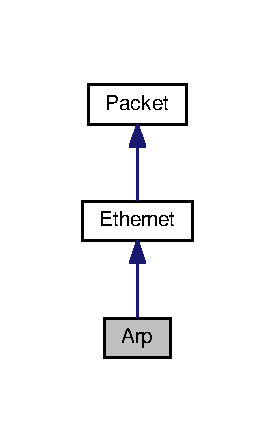
\includegraphics[width=132pt]{class_arp__inherit__graph}
\end{center}
\end{figure}


Collaboration diagram for Arp\-:\nopagebreak
\begin{figure}[H]
\begin{center}
\leavevmode
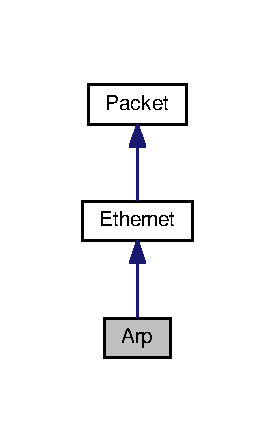
\includegraphics[width=132pt]{class_arp__coll__graph}
\end{center}
\end{figure}
\subsection*{Public Member Functions}
\begin{DoxyCompactItemize}
\item 
\hyperlink{class_arp_a1af9d2c89cc67c74e8621b47f33ae773}{Arp} (pcap\-\_\-t $\ast$device)
\begin{DoxyCompactList}\small\item\em \hyperlink{class_arp}{Arp} Constructor. \hyperlink{class_arp}{Arp} class's constructor. \end{DoxyCompactList}\item 
\hyperlink{structuchar_mac}{uchar\-Mac} \hyperlink{class_arp_adc3ecc7bcb032b6a352ac9867ae75766}{get\-Src\-Arp\-Mac} ()
\begin{DoxyCompactList}\small\item\em Accessor on source mac. \end{DoxyCompactList}\item 
\hyperlink{structuchar_mac}{uchar\-Mac} \hyperlink{class_arp_aaa4f036bf6ad3a85cced8ddc66872c09}{get\-Dst\-Arp\-Mac} ()
\begin{DoxyCompactList}\small\item\em Accessor on destination mac. \end{DoxyCompactList}\item 
uint16\-\_\-t \hyperlink{class_arp_ae8ab693dbb641210a70aa4d8ee76a722}{get\-Op} ()
\begin{DoxyCompactList}\small\item\em Accessor on \hyperlink{class_arp}{Arp}'s operation type. \end{DoxyCompactList}\item 
void \hyperlink{class_arp_af3bf7936c6fc4312175cad8ab1e88757}{set\-Src\-Arp\-Mac} (const \hyperlink{structuchar_mac}{uchar\-Mac} \&src\-Mac)
\begin{DoxyCompactList}\small\item\em Accessor for set source mac. \end{DoxyCompactList}\item 
void \hyperlink{class_arp_adfe61fa40b101e43e4785ea74a6cf291}{set\-Dst\-Arp\-Mac} (const \hyperlink{structuchar_mac}{uchar\-Mac} \&dst\-Mac)
\begin{DoxyCompactList}\small\item\em Accessor for set destination mac. \end{DoxyCompactList}\item 
void \hyperlink{class_arp_aad6cfb26dca5ea92b4471bec7d61e4e1}{set\-Op} (uint16\-\_\-t op)
\begin{DoxyCompactList}\small\item\em Accessor for set \hyperlink{class_arp}{Arp}'s operation type. \end{DoxyCompactList}\item 
void \hyperlink{class_arp_a80f313738e2521f04739fcb9557c7f39}{set\-Dst\-Ip} (const \hyperlink{structuint8_ip}{uint8\-Ip} \&dst\-Ip)
\begin{DoxyCompactList}\small\item\em Accessor for set I\-P destination. \end{DoxyCompactList}\item 
void \hyperlink{class_arp_a756a8d328a55c227040b82aa962ce3db}{set\-Src\-Ip} (const \hyperlink{structuint8_ip}{uint8\-Ip} \&src\-Ip)
\begin{DoxyCompactList}\small\item\em Accessor for set I\-P source. \end{DoxyCompactList}\item 
virtual int \hyperlink{class_arp_ab636211e774eb61e3eaa890a11145aee}{send} ()
\begin{DoxyCompactList}\small\item\em Function for send packet. \end{DoxyCompactList}\end{DoxyCompactItemize}
\subsection*{Protected Attributes}
\begin{DoxyCompactItemize}
\item 
\hypertarget{class_arp_a156bdff60d6019131e30809a93b13522}{struct ether\-\_\-arp $\ast$ {\bfseries \-\_\-arp}}\label{class_arp_a156bdff60d6019131e30809a93b13522}

\end{DoxyCompactItemize}


\subsection{Detailed Description}
Class header for build A\-R\-P packet. 

\subsection{Constructor \& Destructor Documentation}
\hypertarget{class_arp_a1af9d2c89cc67c74e8621b47f33ae773}{\index{Arp@{Arp}!Arp@{Arp}}
\index{Arp@{Arp}!Arp@{Arp}}
\subsubsection[{Arp}]{\setlength{\rightskip}{0pt plus 5cm}Arp\-::\-Arp (
\begin{DoxyParamCaption}
\item[{pcap\-\_\-t $\ast$}]{device}
\end{DoxyParamCaption}
)}}\label{class_arp_a1af9d2c89cc67c74e8621b47f33ae773}


\hyperlink{class_arp}{Arp} Constructor. \hyperlink{class_arp}{Arp} class's constructor. 


\begin{DoxyParams}{Parameters}
{\em Pointer} & to network interface. \\
\hline
\end{DoxyParams}


\subsection{Member Function Documentation}
\hypertarget{class_arp_aaa4f036bf6ad3a85cced8ddc66872c09}{\index{Arp@{Arp}!get\-Dst\-Arp\-Mac@{get\-Dst\-Arp\-Mac}}
\index{get\-Dst\-Arp\-Mac@{get\-Dst\-Arp\-Mac}!Arp@{Arp}}
\subsubsection[{get\-Dst\-Arp\-Mac}]{\setlength{\rightskip}{0pt plus 5cm}{\bf uchar\-Mac} Arp\-::get\-Dst\-Arp\-Mac (
\begin{DoxyParamCaption}
{}
\end{DoxyParamCaption}
)}}\label{class_arp_aaa4f036bf6ad3a85cced8ddc66872c09}


Accessor on destination mac. 

\begin{DoxyReturn}{Returns}
Return M\-A\-C address. 
\end{DoxyReturn}
\hypertarget{class_arp_ae8ab693dbb641210a70aa4d8ee76a722}{\index{Arp@{Arp}!get\-Op@{get\-Op}}
\index{get\-Op@{get\-Op}!Arp@{Arp}}
\subsubsection[{get\-Op}]{\setlength{\rightskip}{0pt plus 5cm}uint16\-\_\-t Arp\-::get\-Op (
\begin{DoxyParamCaption}
{}
\end{DoxyParamCaption}
)}}\label{class_arp_ae8ab693dbb641210a70aa4d8ee76a722}


Accessor on \hyperlink{class_arp}{Arp}'s operation type. 

\begin{DoxyReturn}{Returns}
Return Operation type (answer or request). 
\end{DoxyReturn}
\hypertarget{class_arp_adc3ecc7bcb032b6a352ac9867ae75766}{\index{Arp@{Arp}!get\-Src\-Arp\-Mac@{get\-Src\-Arp\-Mac}}
\index{get\-Src\-Arp\-Mac@{get\-Src\-Arp\-Mac}!Arp@{Arp}}
\subsubsection[{get\-Src\-Arp\-Mac}]{\setlength{\rightskip}{0pt plus 5cm}{\bf uchar\-Mac} Arp\-::get\-Src\-Arp\-Mac (
\begin{DoxyParamCaption}
{}
\end{DoxyParamCaption}
)}}\label{class_arp_adc3ecc7bcb032b6a352ac9867ae75766}


Accessor on source mac. 

\begin{DoxyReturn}{Returns}
Return M\-A\-C address. 
\end{DoxyReturn}
\hypertarget{class_arp_ab636211e774eb61e3eaa890a11145aee}{\index{Arp@{Arp}!send@{send}}
\index{send@{send}!Arp@{Arp}}
\subsubsection[{send}]{\setlength{\rightskip}{0pt plus 5cm}int Arp\-::send (
\begin{DoxyParamCaption}
{}
\end{DoxyParamCaption}
)\hspace{0.3cm}{\ttfamily [virtual]}}}\label{class_arp_ab636211e774eb61e3eaa890a11145aee}


Function for send packet. 

\begin{DoxyReturn}{Returns}
Status (if trame is sended or not). 
\end{DoxyReturn}


Reimplemented from \hyperlink{class_ethernet_a07e05248b744e5b156a21c110dd6777c}{Ethernet}.

\hypertarget{class_arp_adfe61fa40b101e43e4785ea74a6cf291}{\index{Arp@{Arp}!set\-Dst\-Arp\-Mac@{set\-Dst\-Arp\-Mac}}
\index{set\-Dst\-Arp\-Mac@{set\-Dst\-Arp\-Mac}!Arp@{Arp}}
\subsubsection[{set\-Dst\-Arp\-Mac}]{\setlength{\rightskip}{0pt plus 5cm}void Arp\-::set\-Dst\-Arp\-Mac (
\begin{DoxyParamCaption}
\item[{const {\bf uchar\-Mac} \&}]{dst\-Mac}
\end{DoxyParamCaption}
)}}\label{class_arp_adfe61fa40b101e43e4785ea74a6cf291}


Accessor for set destination mac. 


\begin{DoxyParams}{Parameters}
{\em Mac} & address. \\
\hline
\end{DoxyParams}
\hypertarget{class_arp_a80f313738e2521f04739fcb9557c7f39}{\index{Arp@{Arp}!set\-Dst\-Ip@{set\-Dst\-Ip}}
\index{set\-Dst\-Ip@{set\-Dst\-Ip}!Arp@{Arp}}
\subsubsection[{set\-Dst\-Ip}]{\setlength{\rightskip}{0pt plus 5cm}void Arp\-::set\-Dst\-Ip (
\begin{DoxyParamCaption}
\item[{const {\bf uint8\-Ip} \&}]{dst\-Ip}
\end{DoxyParamCaption}
)}}\label{class_arp_a80f313738e2521f04739fcb9557c7f39}


Accessor for set I\-P destination. 


\begin{DoxyParams}{Parameters}
{\em I\-P} & address. \\
\hline
\end{DoxyParams}
\hypertarget{class_arp_aad6cfb26dca5ea92b4471bec7d61e4e1}{\index{Arp@{Arp}!set\-Op@{set\-Op}}
\index{set\-Op@{set\-Op}!Arp@{Arp}}
\subsubsection[{set\-Op}]{\setlength{\rightskip}{0pt plus 5cm}void Arp\-::set\-Op (
\begin{DoxyParamCaption}
\item[{uint16\-\_\-t}]{op}
\end{DoxyParamCaption}
)}}\label{class_arp_aad6cfb26dca5ea92b4471bec7d61e4e1}


Accessor for set \hyperlink{class_arp}{Arp}'s operation type. 


\begin{DoxyParams}{Parameters}
{\em Operation} & value. \\
\hline
\end{DoxyParams}
\hypertarget{class_arp_af3bf7936c6fc4312175cad8ab1e88757}{\index{Arp@{Arp}!set\-Src\-Arp\-Mac@{set\-Src\-Arp\-Mac}}
\index{set\-Src\-Arp\-Mac@{set\-Src\-Arp\-Mac}!Arp@{Arp}}
\subsubsection[{set\-Src\-Arp\-Mac}]{\setlength{\rightskip}{0pt plus 5cm}void Arp\-::set\-Src\-Arp\-Mac (
\begin{DoxyParamCaption}
\item[{const {\bf uchar\-Mac} \&}]{src\-Mac}
\end{DoxyParamCaption}
)}}\label{class_arp_af3bf7936c6fc4312175cad8ab1e88757}


Accessor for set source mac. 


\begin{DoxyParams}{Parameters}
{\em Mac} & address. \\
\hline
\end{DoxyParams}
\hypertarget{class_arp_a756a8d328a55c227040b82aa962ce3db}{\index{Arp@{Arp}!set\-Src\-Ip@{set\-Src\-Ip}}
\index{set\-Src\-Ip@{set\-Src\-Ip}!Arp@{Arp}}
\subsubsection[{set\-Src\-Ip}]{\setlength{\rightskip}{0pt plus 5cm}void Arp\-::set\-Src\-Ip (
\begin{DoxyParamCaption}
\item[{const {\bf uint8\-Ip} \&}]{src\-Ip}
\end{DoxyParamCaption}
)}}\label{class_arp_a756a8d328a55c227040b82aa962ce3db}


Accessor for set I\-P source. 


\begin{DoxyParams}{Parameters}
{\em I\-P} & address. \\
\hline
\end{DoxyParams}


The documentation for this class was generated from the following files\-:\begin{DoxyCompactItemize}
\item 
\hyperlink{_arp_8hpp}{Arp.\-hpp}\item 
\hyperlink{_arp_8cpp}{Arp.\-cpp}\end{DoxyCompactItemize}

\hypertarget{class_arp_spoofing}{\section{Arp\-Spoofing Class Reference}
\label{class_arp_spoofing}\index{Arp\-Spoofing@{Arp\-Spoofing}}
}


Class header for run M\-I\-T\-M attack.  




{\ttfamily \#include $<$Arp\-Spoofing.\-hpp$>$}

\subsection*{Public Member Functions}
\begin{DoxyCompactItemize}
\item 
\hyperlink{class_arp_spoofing_a06af109767827fa14cfcdc4afa90b75c}{Arp\-Spoofing} (char $\ast$iface, char $\ast$target, char $\ast$destination)
\begin{DoxyCompactList}\small\item\em \hyperlink{class_arp_spoofing}{Arp\-Spoofing} Constructor. \hyperlink{class_arp_spoofing}{Arp\-Spoofing} class's constructor. \end{DoxyCompactList}\item 
\hypertarget{class_arp_spoofing_a794353824abaaacbf57ef853d633126f}{void \hyperlink{class_arp_spoofing_a794353824abaaacbf57ef853d633126f}{run} ()}\label{class_arp_spoofing_a794353824abaaacbf57ef853d633126f}

\begin{DoxyCompactList}\small\item\em Run M\-I\-T\-M attack. \end{DoxyCompactList}\end{DoxyCompactItemize}


\subsection{Detailed Description}
Class header for run M\-I\-T\-M attack. 

\subsection{Constructor \& Destructor Documentation}
\hypertarget{class_arp_spoofing_a06af109767827fa14cfcdc4afa90b75c}{\index{Arp\-Spoofing@{Arp\-Spoofing}!Arp\-Spoofing@{Arp\-Spoofing}}
\index{Arp\-Spoofing@{Arp\-Spoofing}!ArpSpoofing@{Arp\-Spoofing}}
\subsubsection[{Arp\-Spoofing}]{\setlength{\rightskip}{0pt plus 5cm}Arp\-Spoofing\-::\-Arp\-Spoofing (
\begin{DoxyParamCaption}
\item[{char $\ast$}]{iface, }
\item[{char $\ast$}]{target, }
\item[{char $\ast$}]{destination}
\end{DoxyParamCaption}
)}}\label{class_arp_spoofing_a06af109767827fa14cfcdc4afa90b75c}


\hyperlink{class_arp_spoofing}{Arp\-Spoofing} Constructor. \hyperlink{class_arp_spoofing}{Arp\-Spoofing} class's constructor. 


\begin{DoxyParams}{Parameters}
{\em iface} & \-: Pointer to network interface. \\
\hline
{\em target} & \-: Target's I\-P. \\
\hline
{\em destination} & \-: I\-P who is hijacked in target's A\-R\-P cache. \\
\hline
\end{DoxyParams}


The documentation for this class was generated from the following files\-:\begin{DoxyCompactItemize}
\item 
\hyperlink{_arp_spoofing_8hpp}{Arp\-Spoofing.\-hpp}\item 
\hyperlink{_arp_spoofing_8cpp}{Arp\-Spoofing.\-cpp}\end{DoxyCompactItemize}

\hypertarget{class_ethernet}{\section{Ethernet Class Reference}
\label{class_ethernet}\index{Ethernet@{Ethernet}}
}


Class header for build \hyperlink{class_ethernet}{Ethernet} packet.  




{\ttfamily \#include $<$Ethernet.\-hpp$>$}



Inheritance diagram for Ethernet\-:\nopagebreak
\begin{figure}[H]
\begin{center}
\leavevmode
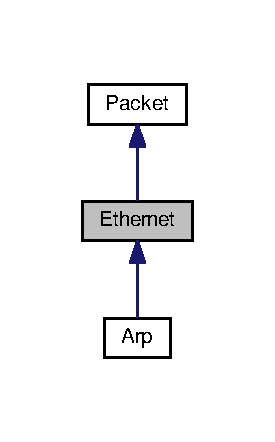
\includegraphics[width=132pt]{class_ethernet__inherit__graph}
\end{center}
\end{figure}


Collaboration diagram for Ethernet\-:\nopagebreak
\begin{figure}[H]
\begin{center}
\leavevmode
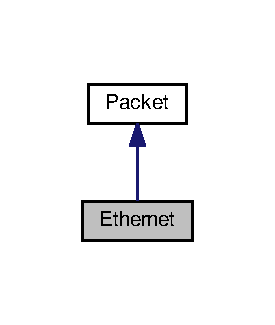
\includegraphics[width=132pt]{class_ethernet__coll__graph}
\end{center}
\end{figure}
\subsection*{Public Member Functions}
\begin{DoxyCompactItemize}
\item 
\hyperlink{class_ethernet_a9daff6153b76200ec40e2a539edca3ac}{Ethernet} (pcap\-\_\-t $\ast$device)
\begin{DoxyCompactList}\small\item\em \hyperlink{class_ethernet}{Ethernet} Constructor. \hyperlink{class_ethernet}{Ethernet} class's constructor. \end{DoxyCompactList}\item 
\hyperlink{structuchar_mac}{uchar\-Mac} \hyperlink{class_ethernet_a81b2d6372c9f5d4a2b8709725df8d7c7}{get\-Src\-Mac} ()
\begin{DoxyCompactList}\small\item\em Accessor on source mac. \end{DoxyCompactList}\item 
\hyperlink{structuchar_mac}{uchar\-Mac} \hyperlink{class_ethernet_ab0d4ec8d1f1f9878660cc425601fa229}{get\-Dst\-Mac} ()
\begin{DoxyCompactList}\small\item\em Accessor on destination mac. \end{DoxyCompactList}\item 
uint16\-\_\-t \hyperlink{class_ethernet_a15f9830364ed2b1197fcd2dab889440d}{get\-Ether\-Type} ()
\begin{DoxyCompactList}\small\item\em Accessor on type of \hyperlink{class_ethernet}{Ethernet} trame. \end{DoxyCompactList}\item 
void \hyperlink{class_ethernet_ad36895e50904c982627f489e3a870b18}{set\-Src\-Mac} (\hyperlink{structuchar_mac}{uchar\-Mac} \&src\-Mac)
\begin{DoxyCompactList}\small\item\em Accessor for set source mac address. \end{DoxyCompactList}\item 
void \hyperlink{class_ethernet_a9d7ea3ce550d82ce0cd1d60b64a96c9c}{set\-Dst\-Mac} (\hyperlink{structuchar_mac}{uchar\-Mac} \&dst\-Mac)
\begin{DoxyCompactList}\small\item\em Accessor for set destination mac address. \end{DoxyCompactList}\item 
void \hyperlink{class_ethernet_ada797dd283c3d976eb78ce4fa9c2184d}{set\-Ether\-Type} (uint16\-\_\-t type)
\begin{DoxyCompactList}\small\item\em Accessor for set \hyperlink{class_ethernet}{Ethernet} trame's type. \end{DoxyCompactList}\item 
virtual int \hyperlink{class_ethernet_a07e05248b744e5b156a21c110dd6777c}{send} ()
\begin{DoxyCompactList}\small\item\em Function for send packet. \end{DoxyCompactList}\end{DoxyCompactItemize}
\subsection*{Protected Attributes}
\begin{DoxyCompactItemize}
\item 
\hypertarget{class_ethernet_ae1141e2b93284fd12aef6212b37fbb04}{struct ether\-\_\-header $\ast$ {\bfseries \-\_\-ethernet}}\label{class_ethernet_ae1141e2b93284fd12aef6212b37fbb04}

\end{DoxyCompactItemize}


\subsection{Detailed Description}
Class header for build \hyperlink{class_ethernet}{Ethernet} packet. 

\subsection{Constructor \& Destructor Documentation}
\hypertarget{class_ethernet_a9daff6153b76200ec40e2a539edca3ac}{\index{Ethernet@{Ethernet}!Ethernet@{Ethernet}}
\index{Ethernet@{Ethernet}!Ethernet@{Ethernet}}
\subsubsection[{Ethernet}]{\setlength{\rightskip}{0pt plus 5cm}Ethernet\-::\-Ethernet (
\begin{DoxyParamCaption}
\item[{pcap\-\_\-t $\ast$}]{device}
\end{DoxyParamCaption}
)}}\label{class_ethernet_a9daff6153b76200ec40e2a539edca3ac}


\hyperlink{class_ethernet}{Ethernet} Constructor. \hyperlink{class_ethernet}{Ethernet} class's constructor. 


\begin{DoxyParams}{Parameters}
{\em Pointer} & to network interface. \\
\hline
\end{DoxyParams}


\subsection{Member Function Documentation}
\hypertarget{class_ethernet_ab0d4ec8d1f1f9878660cc425601fa229}{\index{Ethernet@{Ethernet}!get\-Dst\-Mac@{get\-Dst\-Mac}}
\index{get\-Dst\-Mac@{get\-Dst\-Mac}!Ethernet@{Ethernet}}
\subsubsection[{get\-Dst\-Mac}]{\setlength{\rightskip}{0pt plus 5cm}{\bf uchar\-Mac} Ethernet\-::get\-Dst\-Mac (
\begin{DoxyParamCaption}
{}
\end{DoxyParamCaption}
)}}\label{class_ethernet_ab0d4ec8d1f1f9878660cc425601fa229}


Accessor on destination mac. 

\begin{DoxyReturn}{Returns}
Return M\-A\-C address. 
\end{DoxyReturn}
\hypertarget{class_ethernet_a15f9830364ed2b1197fcd2dab889440d}{\index{Ethernet@{Ethernet}!get\-Ether\-Type@{get\-Ether\-Type}}
\index{get\-Ether\-Type@{get\-Ether\-Type}!Ethernet@{Ethernet}}
\subsubsection[{get\-Ether\-Type}]{\setlength{\rightskip}{0pt plus 5cm}uint16\-\_\-t Ethernet\-::get\-Ether\-Type (
\begin{DoxyParamCaption}
{}
\end{DoxyParamCaption}
)}}\label{class_ethernet_a15f9830364ed2b1197fcd2dab889440d}


Accessor on type of \hyperlink{class_ethernet}{Ethernet} trame. 

\begin{DoxyReturn}{Returns}
Return type value. 
\end{DoxyReturn}
\hypertarget{class_ethernet_a81b2d6372c9f5d4a2b8709725df8d7c7}{\index{Ethernet@{Ethernet}!get\-Src\-Mac@{get\-Src\-Mac}}
\index{get\-Src\-Mac@{get\-Src\-Mac}!Ethernet@{Ethernet}}
\subsubsection[{get\-Src\-Mac}]{\setlength{\rightskip}{0pt plus 5cm}{\bf uchar\-Mac} Ethernet\-::get\-Src\-Mac (
\begin{DoxyParamCaption}
{}
\end{DoxyParamCaption}
)}}\label{class_ethernet_a81b2d6372c9f5d4a2b8709725df8d7c7}


Accessor on source mac. 

\begin{DoxyReturn}{Returns}
Return M\-A\-C address. 
\end{DoxyReturn}
\hypertarget{class_ethernet_a07e05248b744e5b156a21c110dd6777c}{\index{Ethernet@{Ethernet}!send@{send}}
\index{send@{send}!Ethernet@{Ethernet}}
\subsubsection[{send}]{\setlength{\rightskip}{0pt plus 5cm}int Ethernet\-::send (
\begin{DoxyParamCaption}
{}
\end{DoxyParamCaption}
)\hspace{0.3cm}{\ttfamily [virtual]}}}\label{class_ethernet_a07e05248b744e5b156a21c110dd6777c}


Function for send packet. 

\begin{DoxyReturn}{Returns}
Status (if trame is sended or not). 
\end{DoxyReturn}


Reimplemented from \hyperlink{class_packet_aaa29e94af4309658a1244c81f4651b1a}{Packet}.



Reimplemented in \hyperlink{class_arp_ab636211e774eb61e3eaa890a11145aee}{Arp}.

\hypertarget{class_ethernet_a9d7ea3ce550d82ce0cd1d60b64a96c9c}{\index{Ethernet@{Ethernet}!set\-Dst\-Mac@{set\-Dst\-Mac}}
\index{set\-Dst\-Mac@{set\-Dst\-Mac}!Ethernet@{Ethernet}}
\subsubsection[{set\-Dst\-Mac}]{\setlength{\rightskip}{0pt plus 5cm}void Ethernet\-::set\-Dst\-Mac (
\begin{DoxyParamCaption}
\item[{{\bf uchar\-Mac} \&}]{dst\-Mac}
\end{DoxyParamCaption}
)}}\label{class_ethernet_a9d7ea3ce550d82ce0cd1d60b64a96c9c}


Accessor for set destination mac address. 


\begin{DoxyParams}{Parameters}
{\em M\-A\-C} & address. \\
\hline
\end{DoxyParams}
\hypertarget{class_ethernet_ada797dd283c3d976eb78ce4fa9c2184d}{\index{Ethernet@{Ethernet}!set\-Ether\-Type@{set\-Ether\-Type}}
\index{set\-Ether\-Type@{set\-Ether\-Type}!Ethernet@{Ethernet}}
\subsubsection[{set\-Ether\-Type}]{\setlength{\rightskip}{0pt plus 5cm}void Ethernet\-::set\-Ether\-Type (
\begin{DoxyParamCaption}
\item[{uint16\-\_\-t}]{type}
\end{DoxyParamCaption}
)}}\label{class_ethernet_ada797dd283c3d976eb78ce4fa9c2184d}


Accessor for set \hyperlink{class_ethernet}{Ethernet} trame's type. 


\begin{DoxyParams}{Parameters}
{\em \hyperlink{class_ethernet}{Ethernet}} & trame's type value. \\
\hline
\end{DoxyParams}
\hypertarget{class_ethernet_ad36895e50904c982627f489e3a870b18}{\index{Ethernet@{Ethernet}!set\-Src\-Mac@{set\-Src\-Mac}}
\index{set\-Src\-Mac@{set\-Src\-Mac}!Ethernet@{Ethernet}}
\subsubsection[{set\-Src\-Mac}]{\setlength{\rightskip}{0pt plus 5cm}void Ethernet\-::set\-Src\-Mac (
\begin{DoxyParamCaption}
\item[{{\bf uchar\-Mac} \&}]{src\-Mac}
\end{DoxyParamCaption}
)}}\label{class_ethernet_ad36895e50904c982627f489e3a870b18}


Accessor for set source mac address. 


\begin{DoxyParams}{Parameters}
{\em M\-A\-C} & address. \\
\hline
\end{DoxyParams}


The documentation for this class was generated from the following files\-:\begin{DoxyCompactItemize}
\item 
\hyperlink{_ethernet_8hpp}{Ethernet.\-hpp}\item 
\hyperlink{_ethernet_8cpp}{Ethernet.\-cpp}\end{DoxyCompactItemize}

\hypertarget{class_network_utilities}{\section{Network\-Utilities Class Reference}
\label{class_network_utilities}\index{Network\-Utilities@{Network\-Utilities}}
}


Utilities class for implement network functions.  




{\ttfamily \#include $<$Network\-Utilities.\-hpp$>$}

\subsection*{Static Public Member Functions}
\begin{DoxyCompactItemize}
\item 
static \hyperlink{structuchar_mac}{uchar\-Mac} \hyperlink{class_network_utilities_a87db387fab10438ff356516d46486709}{get\-Mac\-Addr} (char $\ast$device)
\begin{DoxyCompactList}\small\item\em Function for get device's M\-A\-C address. \end{DoxyCompactList}\item 
static \hyperlink{structuint8_ip}{uint8\-Ip} \hyperlink{class_network_utilities_a3340be51030cb7994e377ea4be24a5a9}{get\-Ip\-Addr} (char $\ast$device)
\begin{DoxyCompactList}\small\item\em Function for get device's I\-P address. \end{DoxyCompactList}\item 
static void \hyperlink{class_network_utilities_a37f086940e09f6ea44041b687f086ed0}{print\-Uchar\-Mac} (const \hyperlink{structuchar_mac}{uchar\-Mac} \&mac)
\begin{DoxyCompactList}\small\item\em Print M\-A\-C address. \end{DoxyCompactList}\item 
static void \hyperlink{class_network_utilities_a324f12256f9e027a816fd6dd59419f51}{print\-Uint8\-Ip} (const \hyperlink{structuint8_ip}{uint8\-Ip} \&ip)
\begin{DoxyCompactList}\small\item\em Print I\-P address. \end{DoxyCompactList}\end{DoxyCompactItemize}


\subsection{Detailed Description}
Utilities class for implement network functions. 

\subsection{Member Function Documentation}
\hypertarget{class_network_utilities_a3340be51030cb7994e377ea4be24a5a9}{\index{Network\-Utilities@{Network\-Utilities}!get\-Ip\-Addr@{get\-Ip\-Addr}}
\index{get\-Ip\-Addr@{get\-Ip\-Addr}!NetworkUtilities@{Network\-Utilities}}
\subsubsection[{get\-Ip\-Addr}]{\setlength{\rightskip}{0pt plus 5cm}{\bf uint8\-Ip} Network\-Utilities\-::get\-Ip\-Addr (
\begin{DoxyParamCaption}
\item[{char $\ast$}]{device}
\end{DoxyParamCaption}
)\hspace{0.3cm}{\ttfamily [static]}}}\label{class_network_utilities_a3340be51030cb7994e377ea4be24a5a9}


Function for get device's I\-P address. 


\begin{DoxyParams}{Parameters}
{\em Pointer} & to network interface. \\
\hline
\end{DoxyParams}
\begin{DoxyReturn}{Returns}
Return I\-P address. 
\end{DoxyReturn}
\hypertarget{class_network_utilities_a87db387fab10438ff356516d46486709}{\index{Network\-Utilities@{Network\-Utilities}!get\-Mac\-Addr@{get\-Mac\-Addr}}
\index{get\-Mac\-Addr@{get\-Mac\-Addr}!NetworkUtilities@{Network\-Utilities}}
\subsubsection[{get\-Mac\-Addr}]{\setlength{\rightskip}{0pt plus 5cm}{\bf uchar\-Mac} Network\-Utilities\-::get\-Mac\-Addr (
\begin{DoxyParamCaption}
\item[{char $\ast$}]{device}
\end{DoxyParamCaption}
)\hspace{0.3cm}{\ttfamily [static]}}}\label{class_network_utilities_a87db387fab10438ff356516d46486709}


Function for get device's M\-A\-C address. 


\begin{DoxyParams}{Parameters}
{\em Pointer} & to network interface. \\
\hline
\end{DoxyParams}
\begin{DoxyReturn}{Returns}
Return M\-A\-C address. 
\end{DoxyReturn}
\hypertarget{class_network_utilities_a37f086940e09f6ea44041b687f086ed0}{\index{Network\-Utilities@{Network\-Utilities}!print\-Uchar\-Mac@{print\-Uchar\-Mac}}
\index{print\-Uchar\-Mac@{print\-Uchar\-Mac}!NetworkUtilities@{Network\-Utilities}}
\subsubsection[{print\-Uchar\-Mac}]{\setlength{\rightskip}{0pt plus 5cm}void Network\-Utilities\-::print\-Uchar\-Mac (
\begin{DoxyParamCaption}
\item[{const {\bf uchar\-Mac} \&}]{mac}
\end{DoxyParamCaption}
)\hspace{0.3cm}{\ttfamily [static]}}}\label{class_network_utilities_a37f086940e09f6ea44041b687f086ed0}


Print M\-A\-C address. 


\begin{DoxyParams}{Parameters}
{\em Pointer} & to network interface. \\
\hline
\end{DoxyParams}
\hypertarget{class_network_utilities_a324f12256f9e027a816fd6dd59419f51}{\index{Network\-Utilities@{Network\-Utilities}!print\-Uint8\-Ip@{print\-Uint8\-Ip}}
\index{print\-Uint8\-Ip@{print\-Uint8\-Ip}!NetworkUtilities@{Network\-Utilities}}
\subsubsection[{print\-Uint8\-Ip}]{\setlength{\rightskip}{0pt plus 5cm}void Network\-Utilities\-::print\-Uint8\-Ip (
\begin{DoxyParamCaption}
\item[{const {\bf uint8\-Ip} \&}]{ip}
\end{DoxyParamCaption}
)\hspace{0.3cm}{\ttfamily [static]}}}\label{class_network_utilities_a324f12256f9e027a816fd6dd59419f51}


Print I\-P address. 


\begin{DoxyParams}{Parameters}
{\em Pointer} & to network interface. \\
\hline
\end{DoxyParams}


The documentation for this class was generated from the following files\-:\begin{DoxyCompactItemize}
\item 
\hyperlink{_network_utilities_8hpp}{Network\-Utilities.\-hpp}\item 
\hyperlink{_network_utilities_8cpp}{Network\-Utilities.\-cpp}\end{DoxyCompactItemize}

\hypertarget{class_packet}{\section{Packet Class Reference}
\label{class_packet}\index{Packet@{Packet}}
}


Class header for build network packet.  




{\ttfamily \#include $<$Packet.\-hpp$>$}



Inheritance diagram for Packet\-:\nopagebreak
\begin{figure}[H]
\begin{center}
\leavevmode
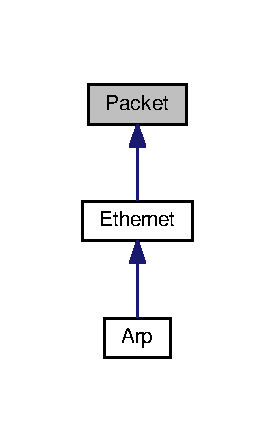
\includegraphics[width=132pt]{class_packet__inherit__graph}
\end{center}
\end{figure}
\subsection*{Public Member Functions}
\begin{DoxyCompactItemize}
\item 
\hyperlink{class_packet_ab3787246de4ff026540b4f1fd91069d9}{Packet} (pcap\-\_\-t $\ast$device)
\begin{DoxyCompactList}\small\item\em \hyperlink{class_packet}{Packet} Constructor. \hyperlink{class_packet}{Packet} class's constructor. \end{DoxyCompactList}\item 
virtual int \hyperlink{class_packet_aaa29e94af4309658a1244c81f4651b1a}{send} ()
\begin{DoxyCompactList}\small\item\em Function for send packet. \end{DoxyCompactList}\end{DoxyCompactItemize}
\subsection*{Protected Attributes}
\begin{DoxyCompactItemize}
\item 
\hypertarget{class_packet_a1aaa10a8ae525113c52c4b3ab5b589fb}{pcap\-\_\-t $\ast$ {\bfseries \-\_\-device}}\label{class_packet_a1aaa10a8ae525113c52c4b3ab5b589fb}

\end{DoxyCompactItemize}


\subsection{Detailed Description}
Class header for build network packet. 

\subsection{Constructor \& Destructor Documentation}
\hypertarget{class_packet_ab3787246de4ff026540b4f1fd91069d9}{\index{Packet@{Packet}!Packet@{Packet}}
\index{Packet@{Packet}!Packet@{Packet}}
\subsubsection[{Packet}]{\setlength{\rightskip}{0pt plus 5cm}Packet\-::\-Packet (
\begin{DoxyParamCaption}
\item[{pcap\-\_\-t $\ast$}]{device}
\end{DoxyParamCaption}
)}}\label{class_packet_ab3787246de4ff026540b4f1fd91069d9}


\hyperlink{class_packet}{Packet} Constructor. \hyperlink{class_packet}{Packet} class's constructor. 


\begin{DoxyParams}{Parameters}
{\em Pointer} & to network interface. \\
\hline
\end{DoxyParams}


\subsection{Member Function Documentation}
\hypertarget{class_packet_aaa29e94af4309658a1244c81f4651b1a}{\index{Packet@{Packet}!send@{send}}
\index{send@{send}!Packet@{Packet}}
\subsubsection[{send}]{\setlength{\rightskip}{0pt plus 5cm}int Packet\-::send (
\begin{DoxyParamCaption}
{}
\end{DoxyParamCaption}
)\hspace{0.3cm}{\ttfamily [virtual]}}}\label{class_packet_aaa29e94af4309658a1244c81f4651b1a}


Function for send packet. 

\begin{DoxyReturn}{Returns}
Status (if trame is sended or not). 
\end{DoxyReturn}


Reimplemented in \hyperlink{class_arp_ab636211e774eb61e3eaa890a11145aee}{Arp}, and \hyperlink{class_ethernet_a07e05248b744e5b156a21c110dd6777c}{Ethernet}.



The documentation for this class was generated from the following files\-:\begin{DoxyCompactItemize}
\item 
\hyperlink{_packet_8hpp}{Packet.\-hpp}\item 
\hyperlink{_packet_8cpp}{Packet.\-cpp}\end{DoxyCompactItemize}

\hypertarget{structuchar_mac}{\section{uchar\-Mac Struct Reference}
\label{structuchar_mac}\index{uchar\-Mac@{uchar\-Mac}}
}
\subsection*{Public Attributes}
\begin{DoxyCompactItemize}
\item 
\hypertarget{structuchar_mac_ac775618c11156b0c2d0d8877c496870e}{u\-\_\-char {\bfseries datas} \mbox{[}6\mbox{]}}\label{structuchar_mac_ac775618c11156b0c2d0d8877c496870e}

\end{DoxyCompactItemize}


The documentation for this struct was generated from the following file\-:\begin{DoxyCompactItemize}
\item 
\hyperlink{_types_8hpp}{Types.\-hpp}\end{DoxyCompactItemize}

\hypertarget{structuint8_ip}{\section{uint8\-Ip Struct Reference}
\label{structuint8_ip}\index{uint8\-Ip@{uint8\-Ip}}
}
\subsection*{Public Attributes}
\begin{DoxyCompactItemize}
\item 
\hypertarget{structuint8_ip_ae324b2b70e65404b606fbcb9e2df1540}{uint8\-\_\-t {\bfseries datas} \mbox{[}4\mbox{]}}\label{structuint8_ip_ae324b2b70e65404b606fbcb9e2df1540}

\end{DoxyCompactItemize}


The documentation for this struct was generated from the following file\-:\begin{DoxyCompactItemize}
\item 
\hyperlink{_types_8hpp}{Types.\-hpp}\end{DoxyCompactItemize}

\chapter{File Documentation}
\hypertarget{_arp_8cpp}{\section{Arp.\-cpp File Reference}
\label{_arp_8cpp}\index{Arp.\-cpp@{Arp.\-cpp}}
}


Class for build A\-R\-P packet.  


{\ttfamily \#include \char`\"{}Arp.\-hpp\char`\"{}}\\*
Include dependency graph for Arp.\-cpp\-:\nopagebreak
\begin{figure}[H]
\begin{center}
\leavevmode
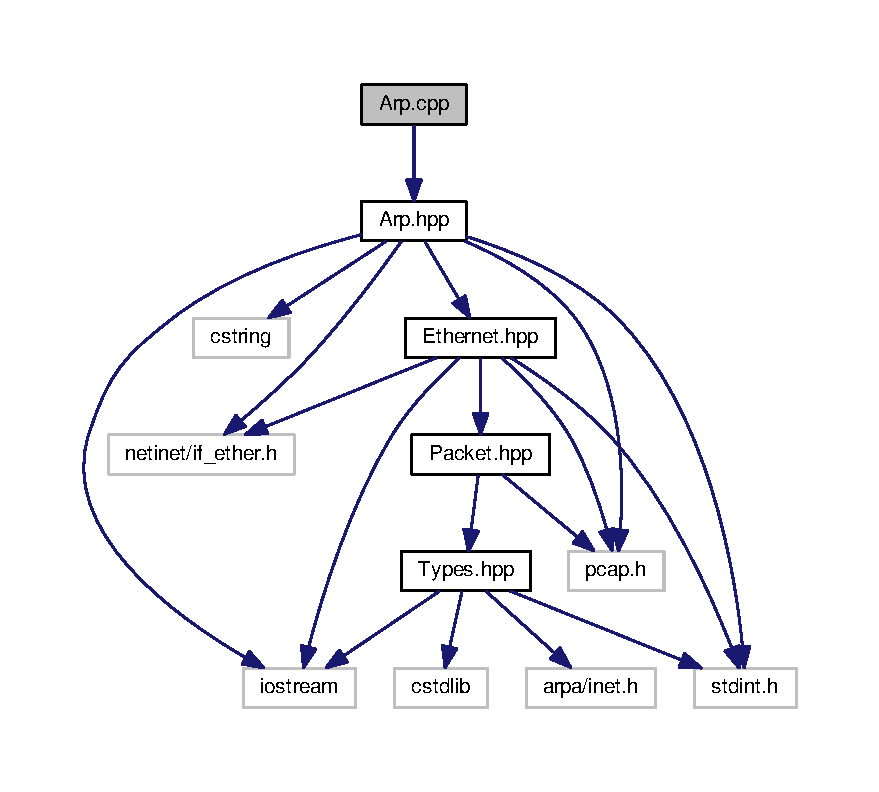
\includegraphics[width=350pt]{_arp_8cpp__incl}
\end{center}
\end{figure}


\subsection{Detailed Description}
Class for build A\-R\-P packet. \begin{DoxyAuthor}{Author}
Jeremy Z\-Y\-R\-A 
\end{DoxyAuthor}
\begin{DoxyVersion}{Version}
1.\-0 
\end{DoxyVersion}

\hypertarget{_arp_8hpp}{\section{Arp.\-hpp File Reference}
\label{_arp_8hpp}\index{Arp.\-hpp@{Arp.\-hpp}}
}


Class header for build A\-R\-P packet.  


{\ttfamily \#include $<$iostream$>$}\\*
{\ttfamily \#include $<$cstring$>$}\\*
{\ttfamily \#include $<$stdint.\-h$>$}\\*
{\ttfamily \#include $<$pcap.\-h$>$}\\*
{\ttfamily \#include $<$netinet/if\-\_\-ether.\-h$>$}\\*
{\ttfamily \#include \char`\"{}Ethernet.\-hpp\char`\"{}}\\*
Include dependency graph for Arp.\-hpp\-:\nopagebreak
\begin{figure}[H]
\begin{center}
\leavevmode
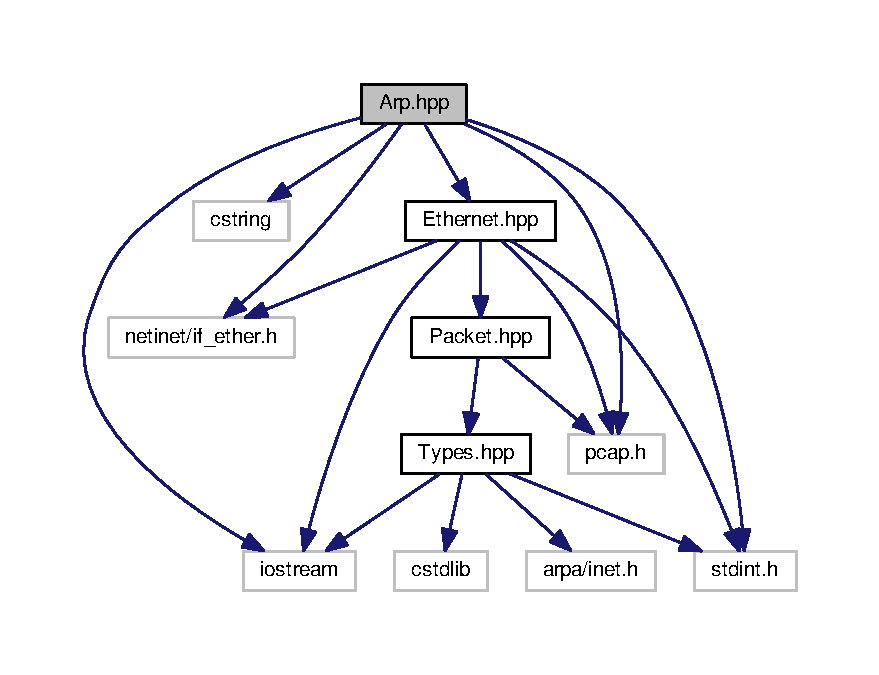
\includegraphics[width=350pt]{_arp_8hpp__incl}
\end{center}
\end{figure}
This graph shows which files directly or indirectly include this file\-:\nopagebreak
\begin{figure}[H]
\begin{center}
\leavevmode
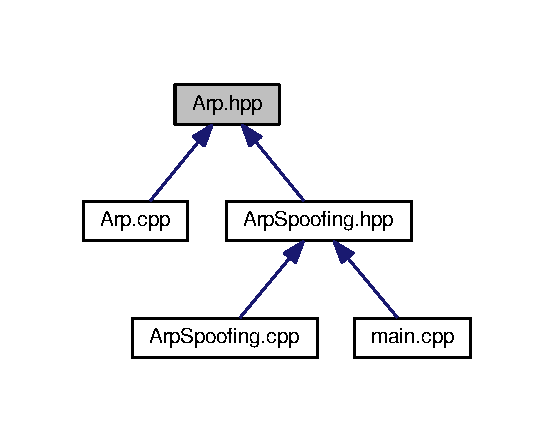
\includegraphics[width=266pt]{_arp_8hpp__dep__incl}
\end{center}
\end{figure}
\subsection*{Classes}
\begin{DoxyCompactItemize}
\item 
class \hyperlink{class_arp}{Arp}
\begin{DoxyCompactList}\small\item\em Class header for build A\-R\-P packet. \end{DoxyCompactList}\end{DoxyCompactItemize}


\subsection{Detailed Description}
Class header for build A\-R\-P packet. \begin{DoxyAuthor}{Author}
Jeremy Z\-Y\-R\-A 
\end{DoxyAuthor}
\begin{DoxyVersion}{Version}
1.\-0 
\end{DoxyVersion}

\hypertarget{_arp_spoofing_8cpp}{\section{Arp\-Spoofing.\-cpp File Reference}
\label{_arp_spoofing_8cpp}\index{Arp\-Spoofing.\-cpp@{Arp\-Spoofing.\-cpp}}
}


Class for run M\-I\-T\-M attack.  


{\ttfamily \#include \char`\"{}Arp\-Spoofing.\-hpp\char`\"{}}\\*
Include dependency graph for Arp\-Spoofing.\-cpp\-:\nopagebreak
\begin{figure}[H]
\begin{center}
\leavevmode
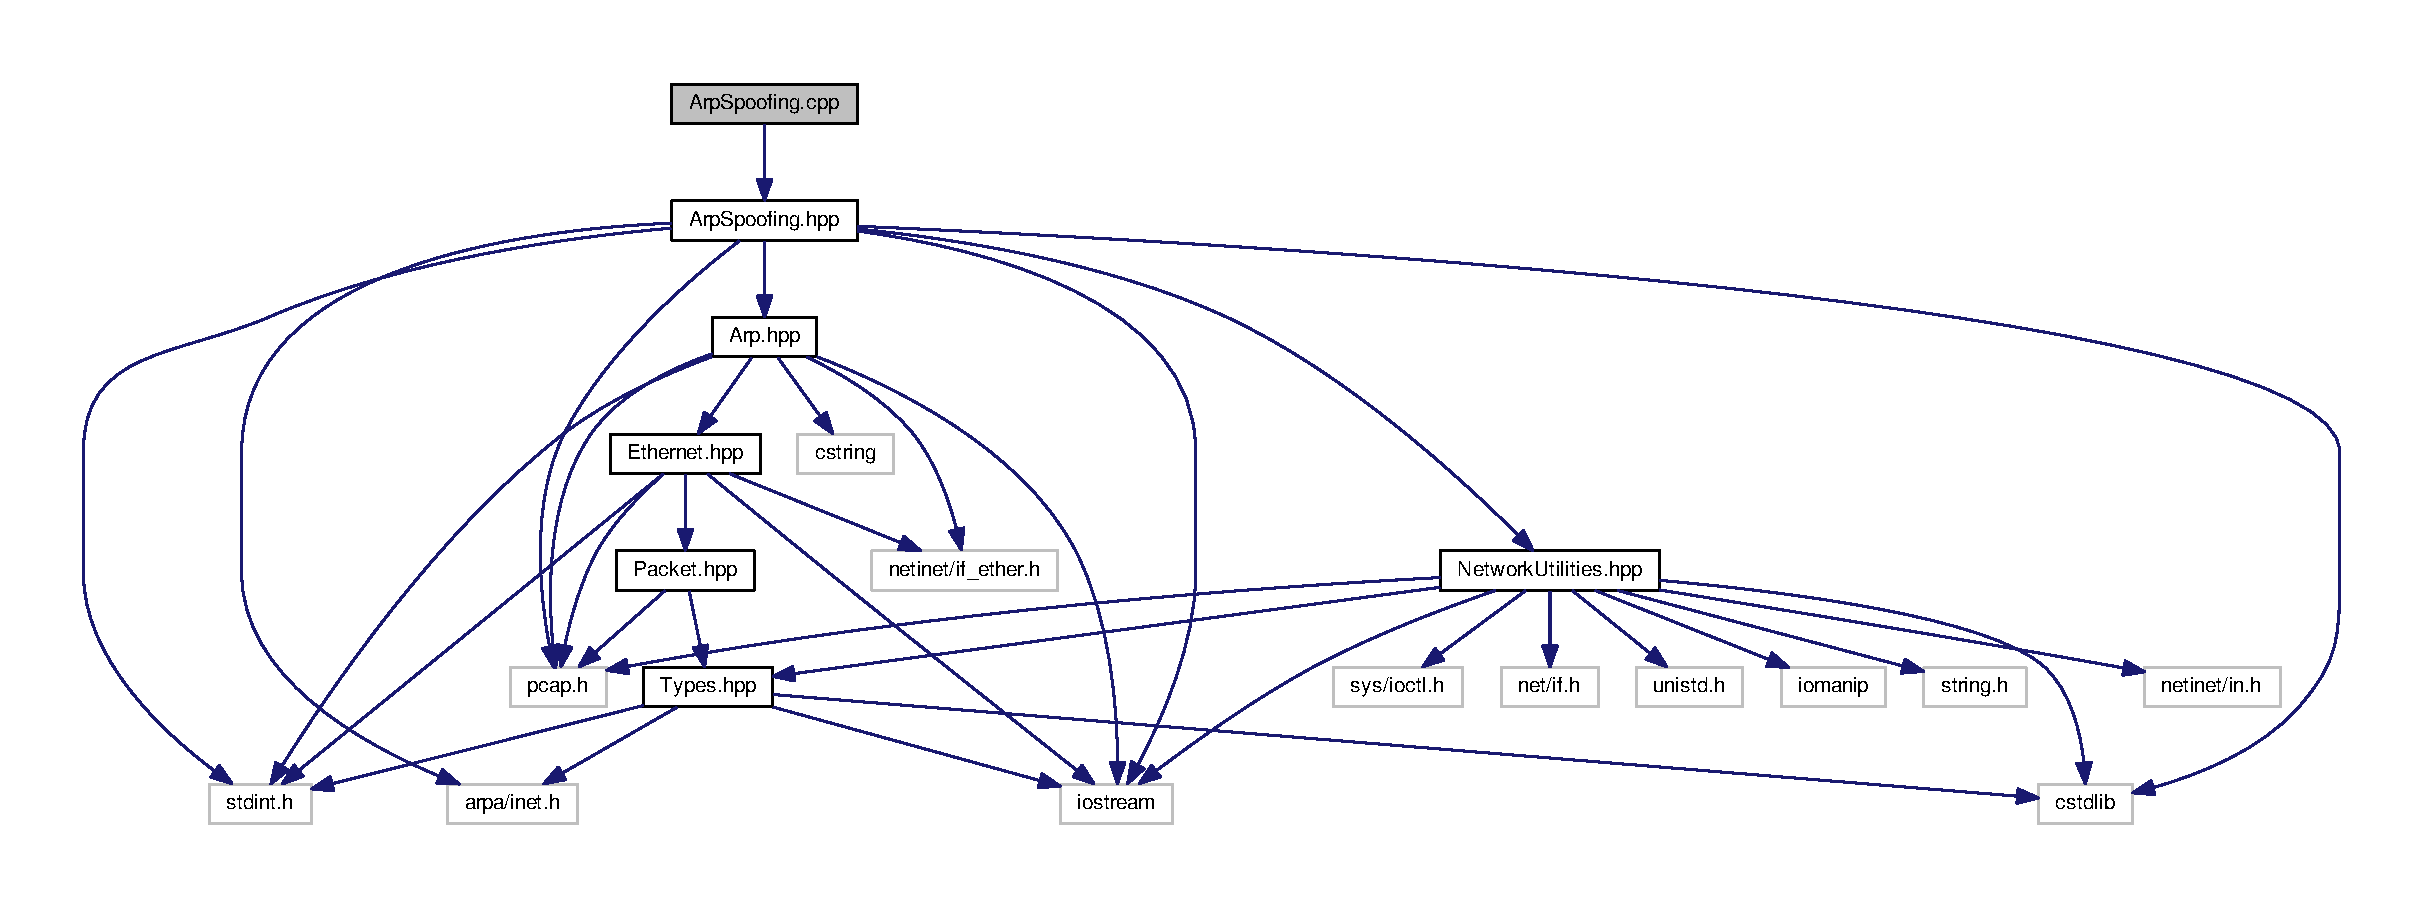
\includegraphics[width=350pt]{_arp_spoofing_8cpp__incl}
\end{center}
\end{figure}


\subsection{Detailed Description}
Class for run M\-I\-T\-M attack. \begin{DoxyAuthor}{Author}
Jeremy Z\-Y\-R\-A 
\end{DoxyAuthor}
\begin{DoxyVersion}{Version}
1.\-0 
\end{DoxyVersion}

\hypertarget{_arp_spoofing_8hpp}{\section{Arp\-Spoofing.\-hpp File Reference}
\label{_arp_spoofing_8hpp}\index{Arp\-Spoofing.\-hpp@{Arp\-Spoofing.\-hpp}}
}


Class header for run M\-I\-T\-M attack.  


{\ttfamily \#include $<$iostream$>$}\\*
{\ttfamily \#include $<$cstdlib$>$}\\*
{\ttfamily \#include $<$pcap.\-h$>$}\\*
{\ttfamily \#include $<$stdint.\-h$>$}\\*
{\ttfamily \#include $<$arpa/inet.\-h$>$}\\*
{\ttfamily \#include \char`\"{}Arp.\-hpp\char`\"{}}\\*
{\ttfamily \#include \char`\"{}Network\-Utilities.\-hpp\char`\"{}}\\*
Include dependency graph for Arp\-Spoofing.\-hpp\-:\nopagebreak
\begin{figure}[H]
\begin{center}
\leavevmode
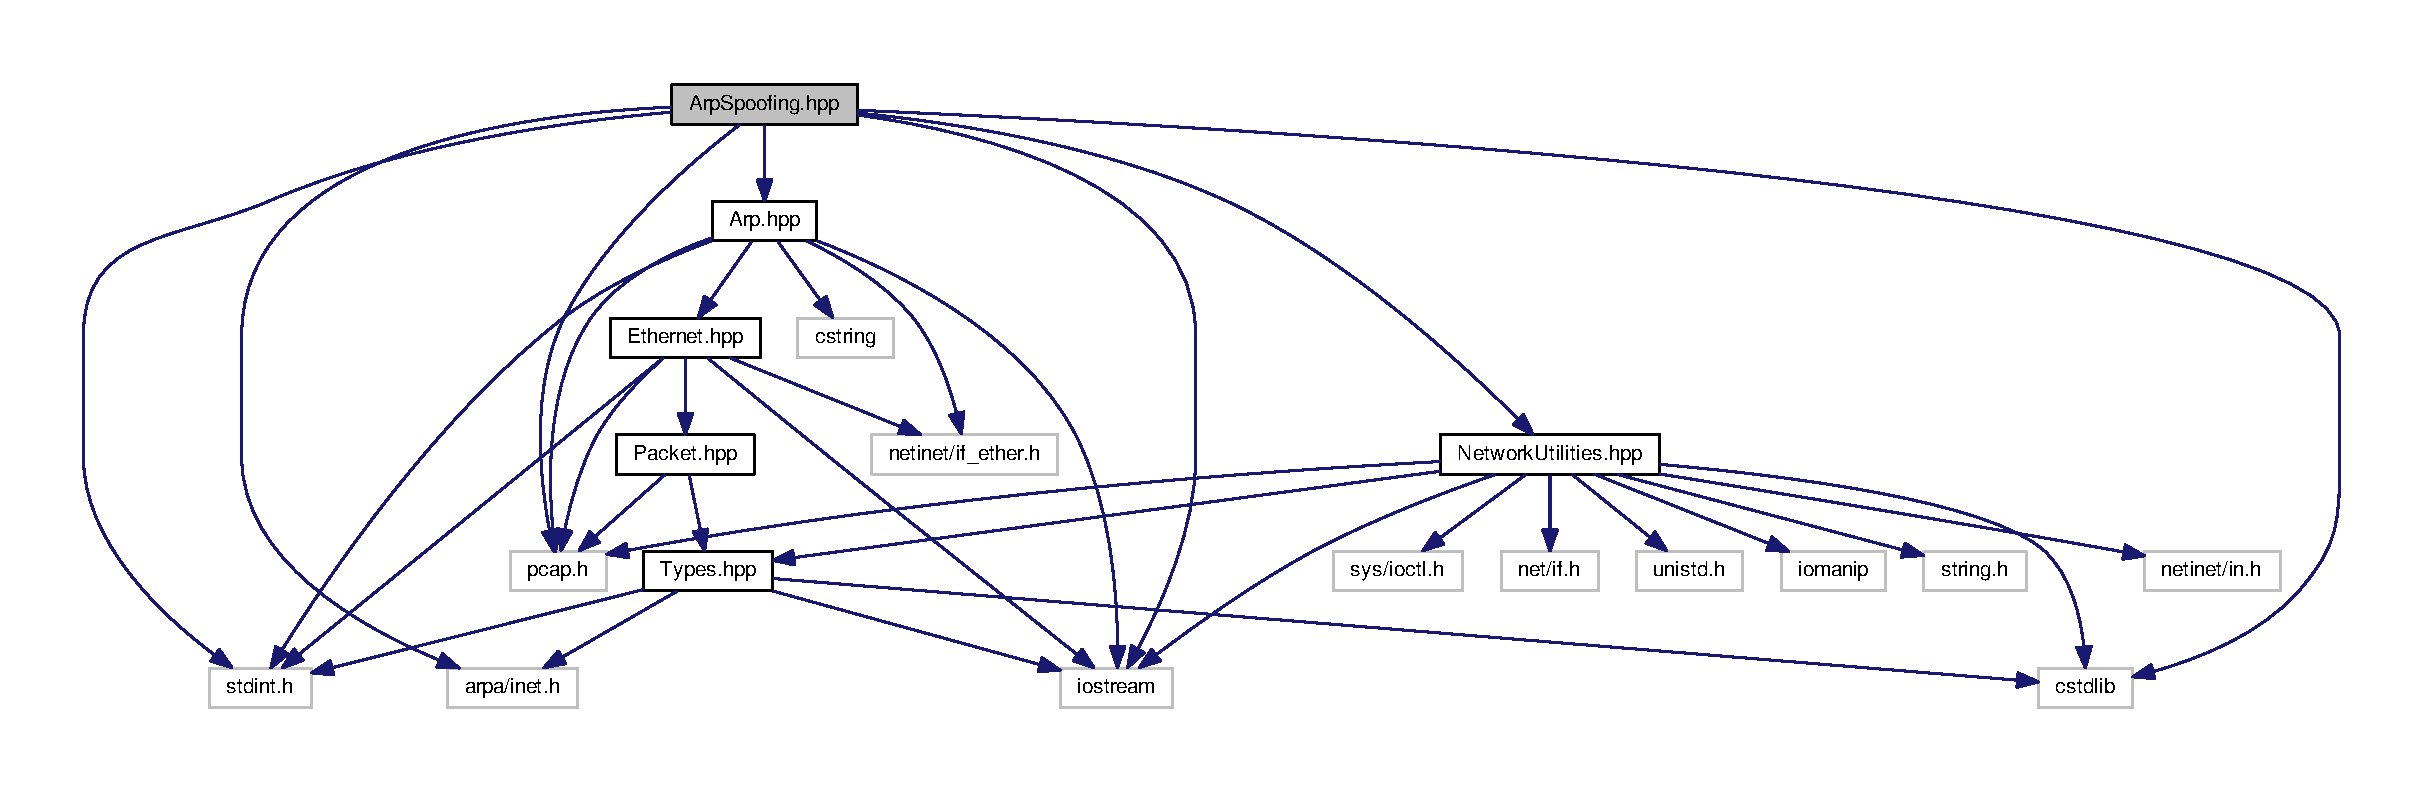
\includegraphics[width=350pt]{_arp_spoofing_8hpp__incl}
\end{center}
\end{figure}
This graph shows which files directly or indirectly include this file\-:\nopagebreak
\begin{figure}[H]
\begin{center}
\leavevmode
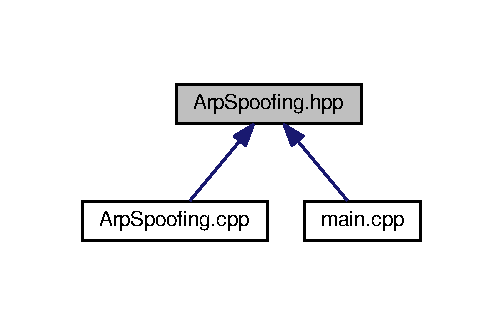
\includegraphics[width=242pt]{_arp_spoofing_8hpp__dep__incl}
\end{center}
\end{figure}
\subsection*{Classes}
\begin{DoxyCompactItemize}
\item 
class \hyperlink{class_arp_spoofing}{Arp\-Spoofing}
\begin{DoxyCompactList}\small\item\em Class header for run M\-I\-T\-M attack. \end{DoxyCompactList}\end{DoxyCompactItemize}
\subsection*{Macros}
\begin{DoxyCompactItemize}
\item 
\hypertarget{_arp_spoofing_8hpp_aebdc7d8ca8e25ed8efc90bb88ef7ef5b}{\#define {\bfseries P\-A\-C\-K\-E\-T\-\_\-\-S\-I\-Z\-E}~65536}\label{_arp_spoofing_8hpp_aebdc7d8ca8e25ed8efc90bb88ef7ef5b}

\item 
\hypertarget{_arp_spoofing_8hpp_a53bb6ce0dbc843daa4ad914d78713ac2}{\#define {\bfseries T\-I\-M\-E\-O\-U\-T\-\_\-\-M\-S}~3000}\label{_arp_spoofing_8hpp_a53bb6ce0dbc843daa4ad914d78713ac2}

\item 
\hypertarget{_arp_spoofing_8hpp_a3b6fc65d4c1c940ee1d8b00a767d2c98}{\#define {\bfseries P\-R\-O\-M\-I\-S\-C\-\_\-\-M\-O\-D\-E}~0}\label{_arp_spoofing_8hpp_a3b6fc65d4c1c940ee1d8b00a767d2c98}

\item 
\hypertarget{_arp_spoofing_8hpp_a460b2d55d43010c5271d676751fe2325}{\#define {\bfseries T\-I\-M\-E\-\_\-\-S\-L\-E\-E\-P}~2}\label{_arp_spoofing_8hpp_a460b2d55d43010c5271d676751fe2325}

\end{DoxyCompactItemize}


\subsection{Detailed Description}
Class header for run M\-I\-T\-M attack. \begin{DoxyAuthor}{Author}
Jeremy Z\-Y\-R\-A 
\end{DoxyAuthor}
\begin{DoxyVersion}{Version}
1.\-0 
\end{DoxyVersion}

\hypertarget{_ethernet_8cpp}{\section{Ethernet.\-cpp File Reference}
\label{_ethernet_8cpp}\index{Ethernet.\-cpp@{Ethernet.\-cpp}}
}


Class for build \hyperlink{class_ethernet}{Ethernet} packet.  


{\ttfamily \#include \char`\"{}Ethernet.\-hpp\char`\"{}}\\*
Include dependency graph for Ethernet.\-cpp\-:\nopagebreak
\begin{figure}[H]
\begin{center}
\leavevmode
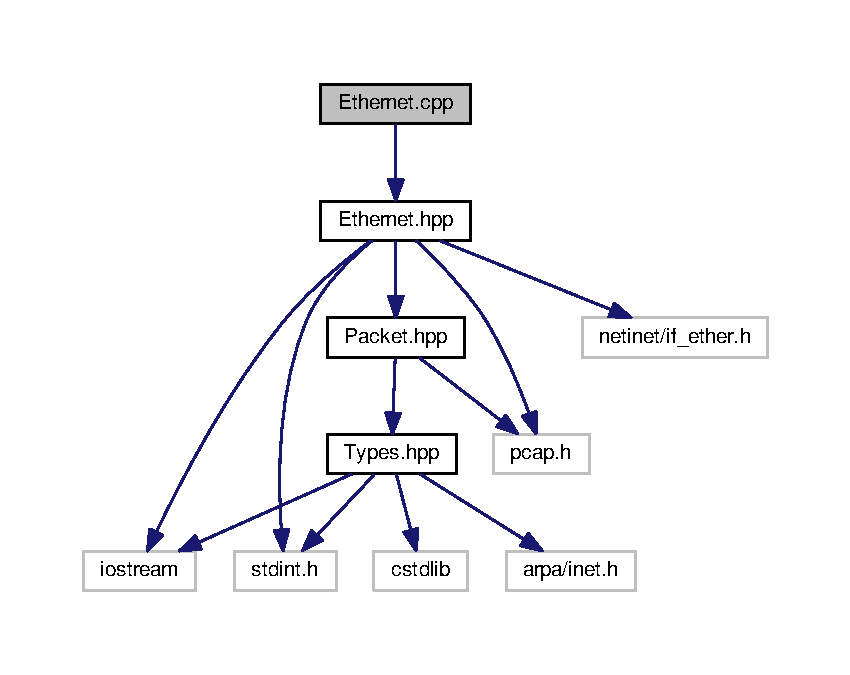
\includegraphics[width=350pt]{_ethernet_8cpp__incl}
\end{center}
\end{figure}


\subsection{Detailed Description}
Class for build \hyperlink{class_ethernet}{Ethernet} packet. \begin{DoxyAuthor}{Author}
Jeremy Z\-Y\-R\-A 
\end{DoxyAuthor}
\begin{DoxyVersion}{Version}
1.\-0 
\end{DoxyVersion}

\hypertarget{_ethernet_8hpp}{\section{Ethernet.\-hpp File Reference}
\label{_ethernet_8hpp}\index{Ethernet.\-hpp@{Ethernet.\-hpp}}
}


Class header for build \hyperlink{class_ethernet}{Ethernet} packet.  


{\ttfamily \#include $<$iostream$>$}\\*
{\ttfamily \#include $<$stdint.\-h$>$}\\*
{\ttfamily \#include $<$pcap.\-h$>$}\\*
{\ttfamily \#include $<$netinet/if\-\_\-ether.\-h$>$}\\*
{\ttfamily \#include \char`\"{}Packet.\-hpp\char`\"{}}\\*
Include dependency graph for Ethernet.\-hpp\-:\nopagebreak
\begin{figure}[H]
\begin{center}
\leavevmode
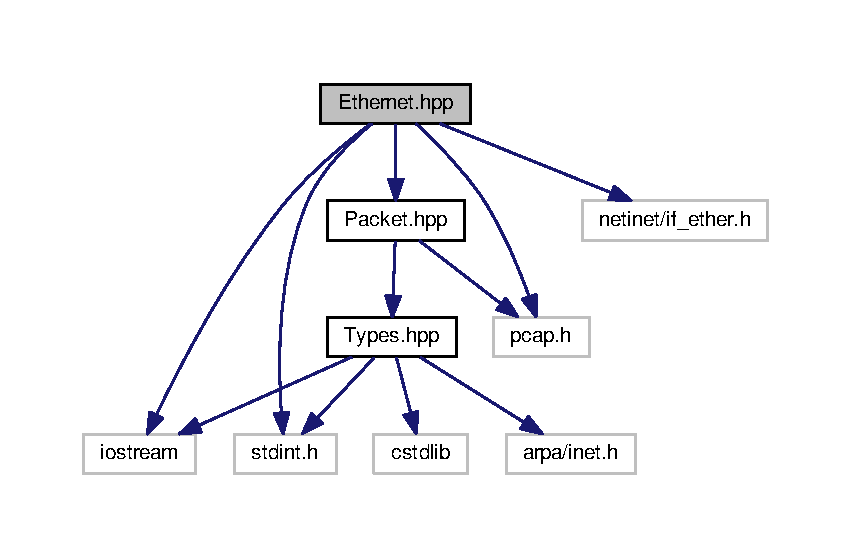
\includegraphics[width=350pt]{_ethernet_8hpp__incl}
\end{center}
\end{figure}
This graph shows which files directly or indirectly include this file\-:\nopagebreak
\begin{figure}[H]
\begin{center}
\leavevmode
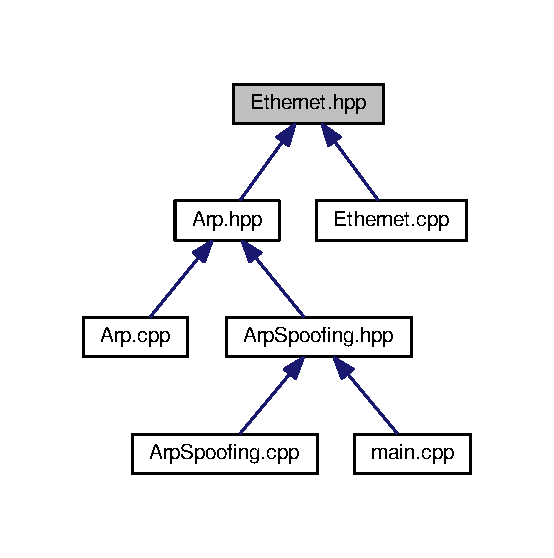
\includegraphics[width=266pt]{_ethernet_8hpp__dep__incl}
\end{center}
\end{figure}
\subsection*{Classes}
\begin{DoxyCompactItemize}
\item 
class \hyperlink{class_ethernet}{Ethernet}
\begin{DoxyCompactList}\small\item\em Class header for build \hyperlink{class_ethernet}{Ethernet} packet. \end{DoxyCompactList}\end{DoxyCompactItemize}


\subsection{Detailed Description}
Class header for build \hyperlink{class_ethernet}{Ethernet} packet. \begin{DoxyAuthor}{Author}
Jeremy Z\-Y\-R\-A 
\end{DoxyAuthor}
\begin{DoxyVersion}{Version}
1.\-0 
\end{DoxyVersion}

\hypertarget{main_8cpp}{\section{main.\-cpp File Reference}
\label{main_8cpp}\index{main.\-cpp@{main.\-cpp}}
}


Program's entry point.  


{\ttfamily \#include $<$iostream$>$}\\*
{\ttfamily \#include $<$pcap.\-h$>$}\\*
{\ttfamily \#include $<$unistd.\-h$>$}\\*
{\ttfamily \#include \char`\"{}Arp\-Spoofing.\-hpp\char`\"{}}\\*
Include dependency graph for main.\-cpp\-:\nopagebreak
\begin{figure}[H]
\begin{center}
\leavevmode
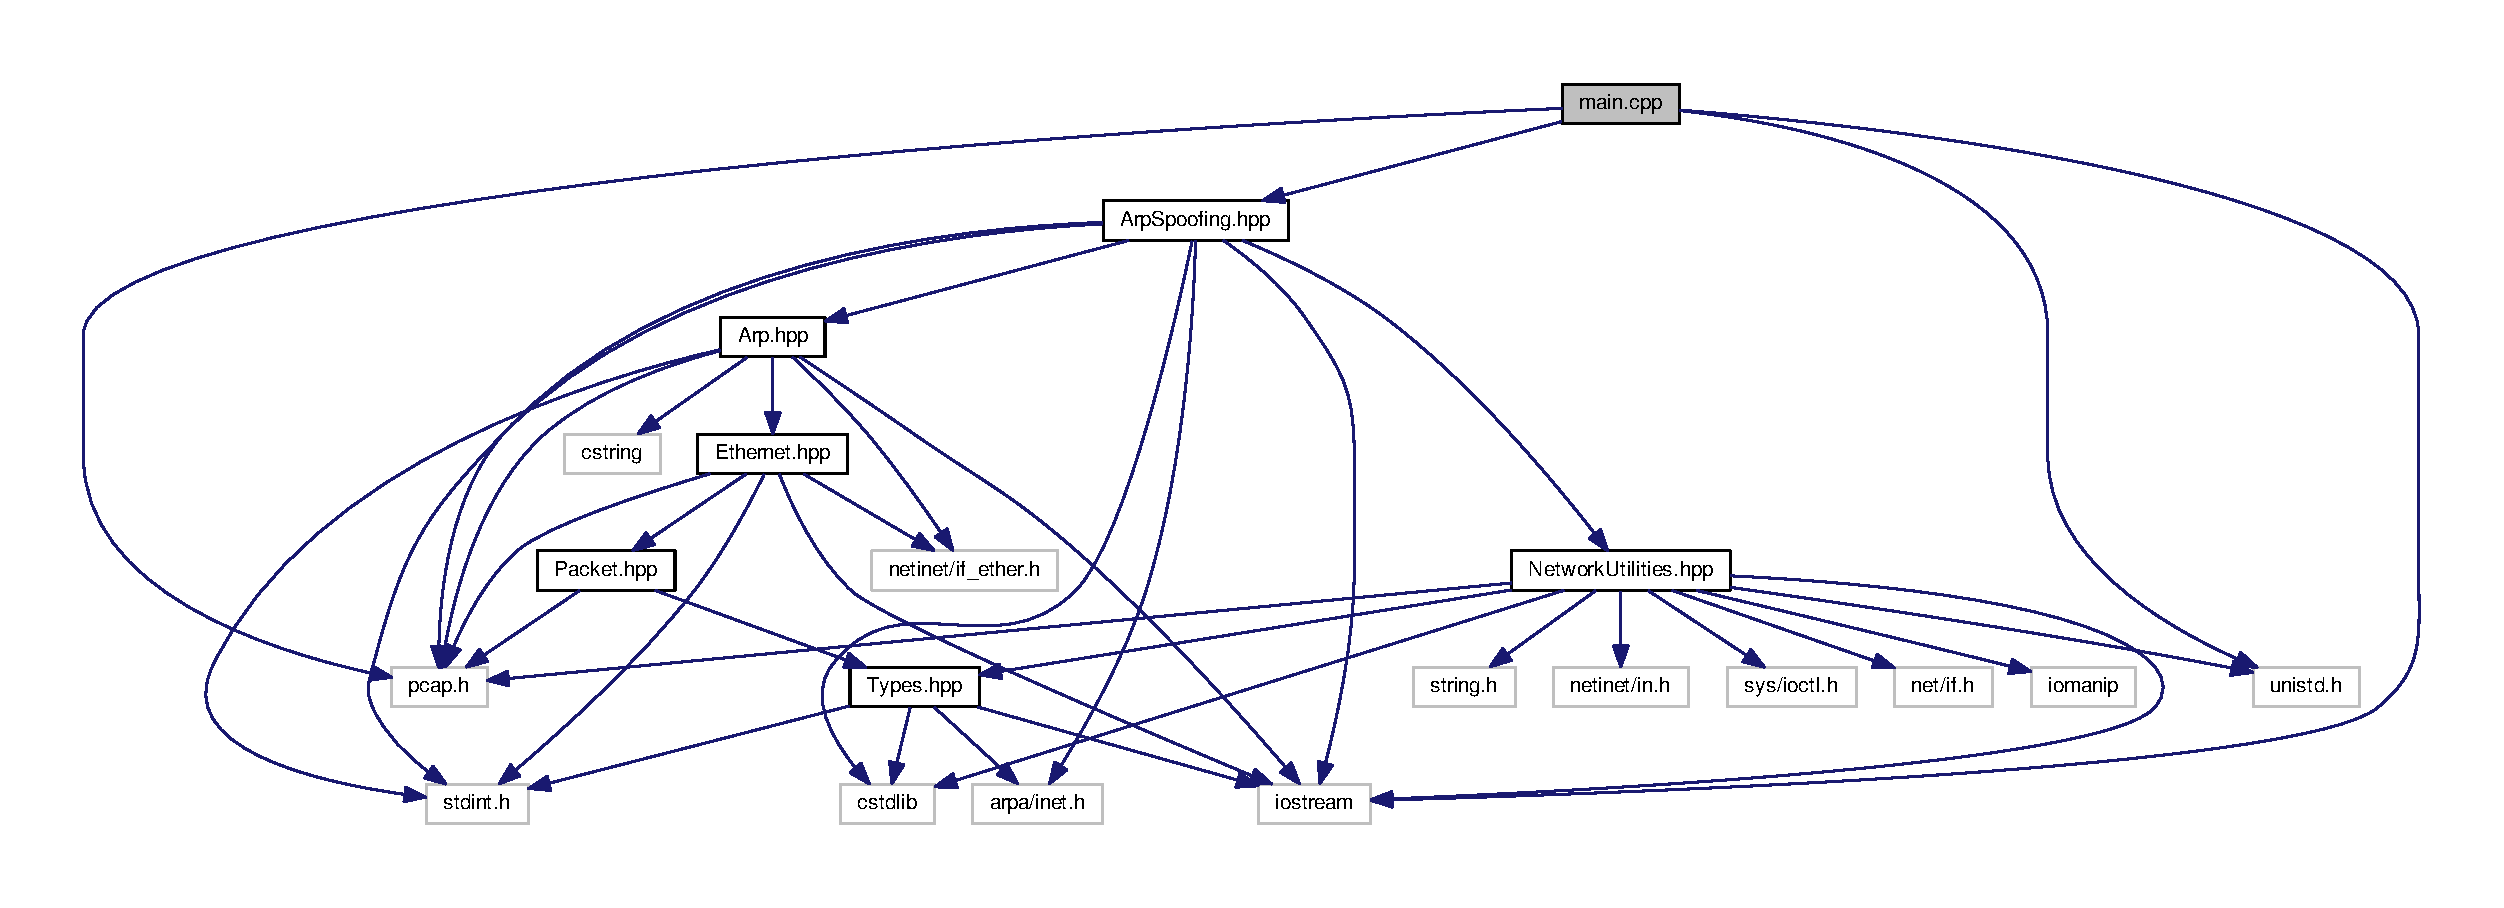
\includegraphics[width=350pt]{main_8cpp__incl}
\end{center}
\end{figure}
\subsection*{Functions}
\begin{DoxyCompactItemize}
\item 
\hypertarget{main_8cpp_ab5a25ef913f5c22270a79d0ea4d89252}{void \hyperlink{main_8cpp_ab5a25ef913f5c22270a79d0ea4d89252}{print\-Usage} (char $\ast$name)}\label{main_8cpp_ab5a25ef913f5c22270a79d0ea4d89252}

\begin{DoxyCompactList}\small\item\em Function for print usage. \end{DoxyCompactList}\item 
\hypertarget{main_8cpp_a0ddf1224851353fc92bfbff6f499fa97}{int \hyperlink{main_8cpp_a0ddf1224851353fc92bfbff6f499fa97}{main} (int argc, char $\ast$argv\mbox{[}$\,$\mbox{]})}\label{main_8cpp_a0ddf1224851353fc92bfbff6f499fa97}

\begin{DoxyCompactList}\small\item\em Program's entry point. \end{DoxyCompactList}\end{DoxyCompactItemize}


\subsection{Detailed Description}
Program's entry point. \begin{DoxyAuthor}{Author}
Jeremy Z\-Y\-R\-A 
\end{DoxyAuthor}

\hypertarget{_network_utilities_8cpp}{\section{Network\-Utilities.\-cpp File Reference}
\label{_network_utilities_8cpp}\index{Network\-Utilities.\-cpp@{Network\-Utilities.\-cpp}}
}


Utilities class for implement network functions.  


{\ttfamily \#include \char`\"{}Network\-Utilities.\-hpp\char`\"{}}\\*
Include dependency graph for Network\-Utilities.\-cpp\-:\nopagebreak
\begin{figure}[H]
\begin{center}
\leavevmode
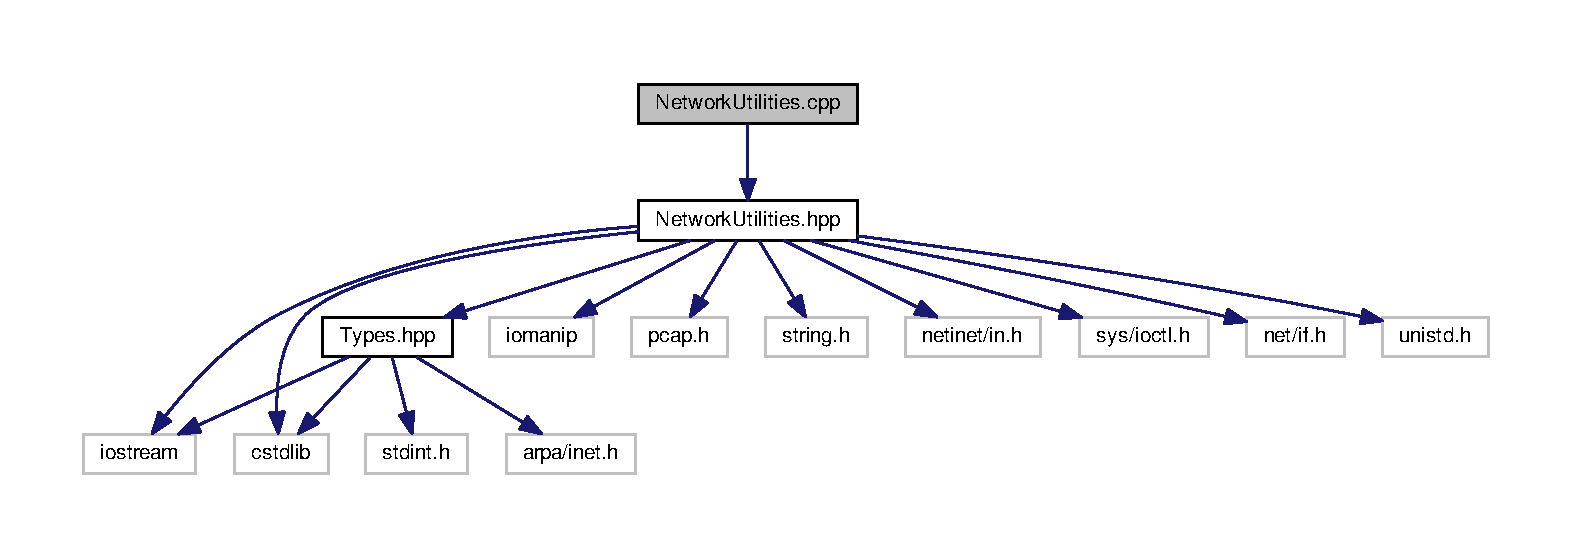
\includegraphics[width=350pt]{_network_utilities_8cpp__incl}
\end{center}
\end{figure}


\subsection{Detailed Description}
Utilities class for implement network functions. \begin{DoxyAuthor}{Author}
Jeremy Z\-Y\-R\-A 
\end{DoxyAuthor}
\begin{DoxyVersion}{Version}
1.\-0 
\end{DoxyVersion}

\hypertarget{_network_utilities_8hpp}{\section{Network\-Utilities.\-hpp File Reference}
\label{_network_utilities_8hpp}\index{Network\-Utilities.\-hpp@{Network\-Utilities.\-hpp}}
}


Utilities class for implement network functions.  


{\ttfamily \#include $<$iostream$>$}\\*
{\ttfamily \#include $<$iomanip$>$}\\*
{\ttfamily \#include $<$pcap.\-h$>$}\\*
{\ttfamily \#include $<$string.\-h$>$}\\*
{\ttfamily \#include $<$netinet/in.\-h$>$}\\*
{\ttfamily \#include $<$sys/ioctl.\-h$>$}\\*
{\ttfamily \#include $<$net/if.\-h$>$}\\*
{\ttfamily \#include $<$unistd.\-h$>$}\\*
{\ttfamily \#include $<$cstdlib$>$}\\*
{\ttfamily \#include \char`\"{}Types.\-hpp\char`\"{}}\\*
Include dependency graph for Network\-Utilities.\-hpp\-:\nopagebreak
\begin{figure}[H]
\begin{center}
\leavevmode
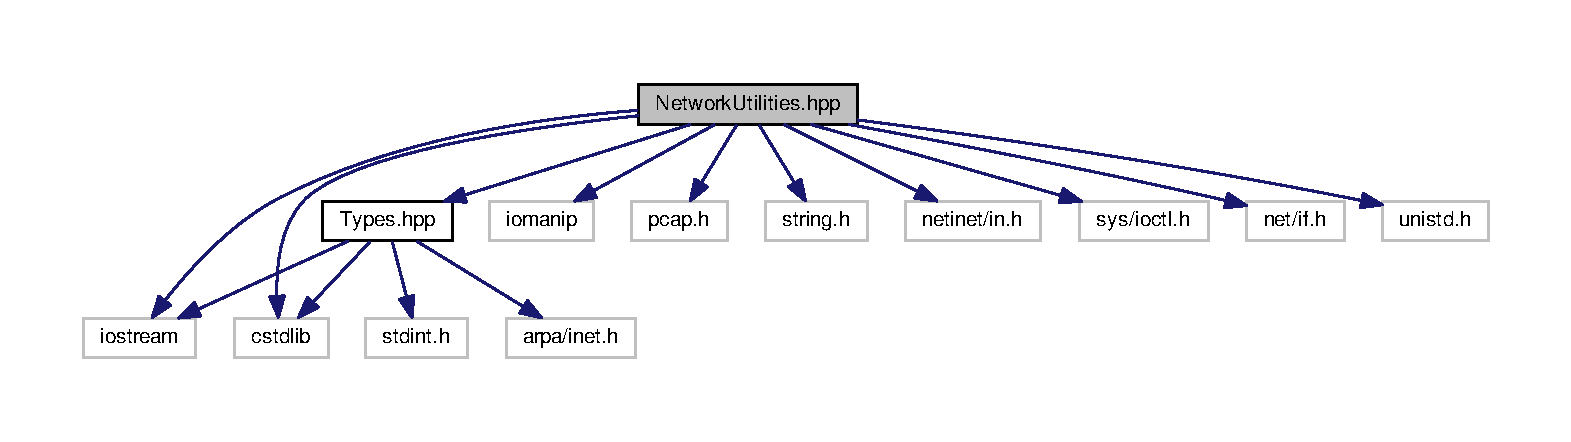
\includegraphics[width=350pt]{_network_utilities_8hpp__incl}
\end{center}
\end{figure}
This graph shows which files directly or indirectly include this file\-:\nopagebreak
\begin{figure}[H]
\begin{center}
\leavevmode
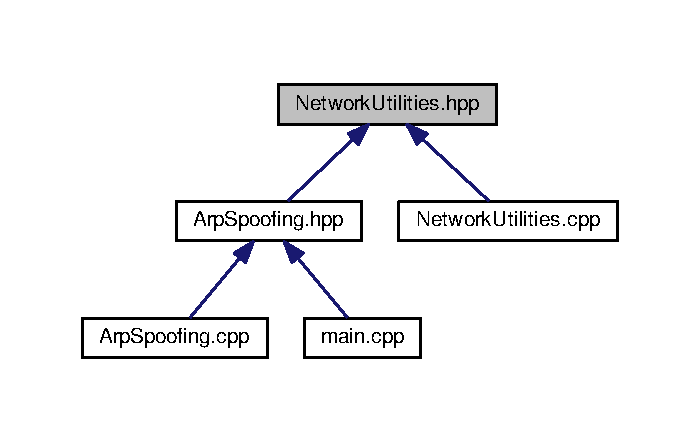
\includegraphics[width=336pt]{_network_utilities_8hpp__dep__incl}
\end{center}
\end{figure}
\subsection*{Classes}
\begin{DoxyCompactItemize}
\item 
class \hyperlink{class_network_utilities}{Network\-Utilities}
\begin{DoxyCompactList}\small\item\em Utilities class for implement network functions. \end{DoxyCompactList}\end{DoxyCompactItemize}


\subsection{Detailed Description}
Utilities class for implement network functions. \begin{DoxyAuthor}{Author}
Jeremy Z\-Y\-R\-A 
\end{DoxyAuthor}
\begin{DoxyVersion}{Version}
1.\-0 
\end{DoxyVersion}

\hypertarget{_packet_8cpp}{\section{Packet.\-cpp File Reference}
\label{_packet_8cpp}\index{Packet.\-cpp@{Packet.\-cpp}}
}


Class for build network packet.  


{\ttfamily \#include \char`\"{}Packet.\-hpp\char`\"{}}\\*
Include dependency graph for Packet.\-cpp\-:\nopagebreak
\begin{figure}[H]
\begin{center}
\leavevmode
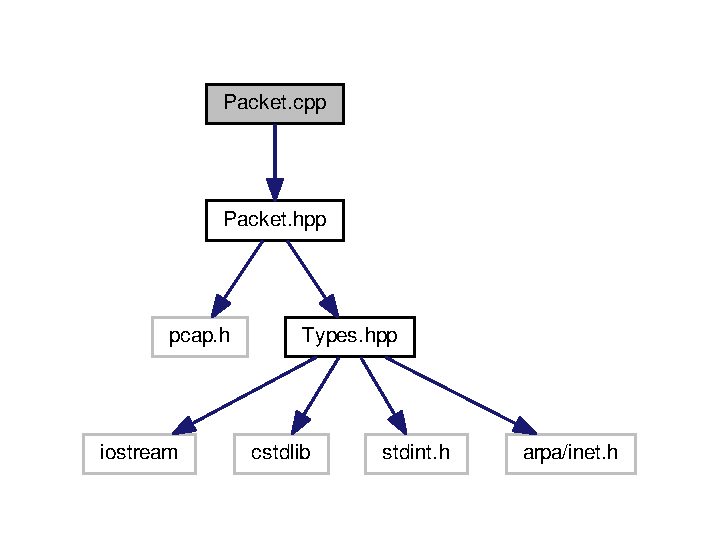
\includegraphics[width=345pt]{_packet_8cpp__incl}
\end{center}
\end{figure}


\subsection{Detailed Description}
Class for build network packet. \begin{DoxyAuthor}{Author}
Jeremy Z\-Y\-R\-A 
\end{DoxyAuthor}
\begin{DoxyVersion}{Version}
1.\-0 
\end{DoxyVersion}

\hypertarget{_packet_8hpp}{\section{Packet.\-hpp File Reference}
\label{_packet_8hpp}\index{Packet.\-hpp@{Packet.\-hpp}}
}


Class header for build network packet.  


{\ttfamily \#include $<$pcap.\-h$>$}\\*
{\ttfamily \#include \char`\"{}Types.\-hpp\char`\"{}}\\*
Include dependency graph for Packet.\-hpp\-:\nopagebreak
\begin{figure}[H]
\begin{center}
\leavevmode
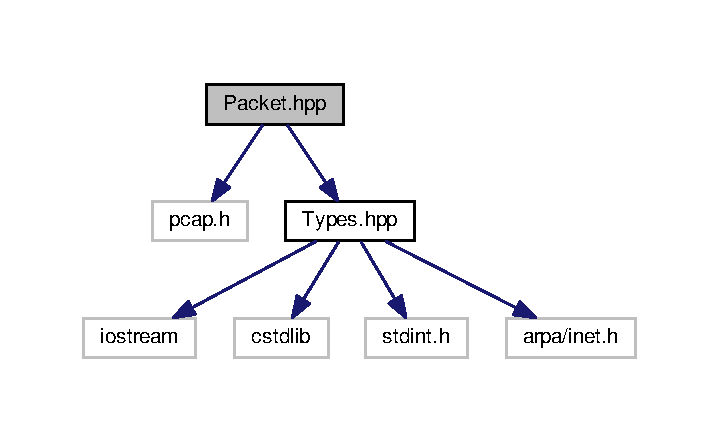
\includegraphics[width=345pt]{_packet_8hpp__incl}
\end{center}
\end{figure}
This graph shows which files directly or indirectly include this file\-:\nopagebreak
\begin{figure}[H]
\begin{center}
\leavevmode
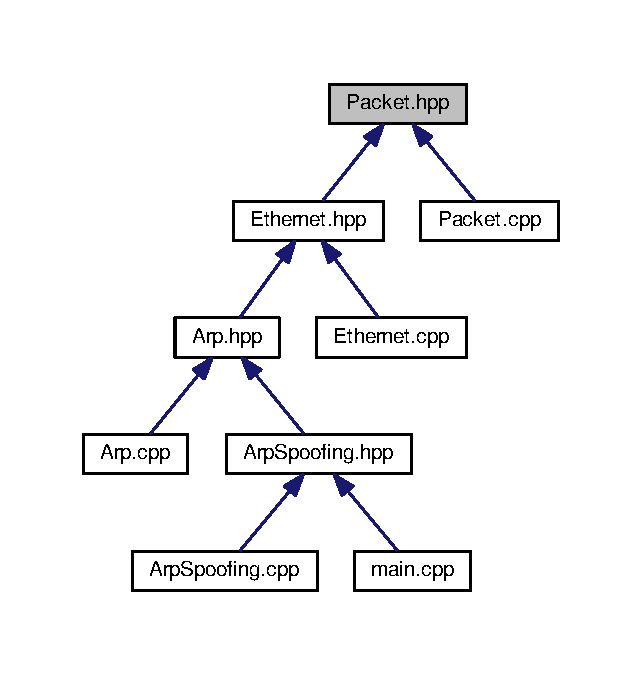
\includegraphics[width=308pt]{_packet_8hpp__dep__incl}
\end{center}
\end{figure}
\subsection*{Classes}
\begin{DoxyCompactItemize}
\item 
class \hyperlink{class_packet}{Packet}
\begin{DoxyCompactList}\small\item\em Class header for build network packet. \end{DoxyCompactList}\end{DoxyCompactItemize}


\subsection{Detailed Description}
Class header for build network packet. \begin{DoxyAuthor}{Author}
Jeremy Z\-Y\-R\-A 
\end{DoxyAuthor}
\begin{DoxyVersion}{Version}
1.\-0 
\end{DoxyVersion}

\hypertarget{_types_8hpp}{\section{Types.\-hpp File Reference}
\label{_types_8hpp}\index{Types.\-hpp@{Types.\-hpp}}
}


Contains definitions of I\-P and M\-A\-C address.  


{\ttfamily \#include $<$iostream$>$}\\*
{\ttfamily \#include $<$cstdlib$>$}\\*
{\ttfamily \#include $<$stdint.\-h$>$}\\*
{\ttfamily \#include $<$arpa/inet.\-h$>$}\\*
Include dependency graph for Types.\-hpp\-:\nopagebreak
\begin{figure}[H]
\begin{center}
\leavevmode
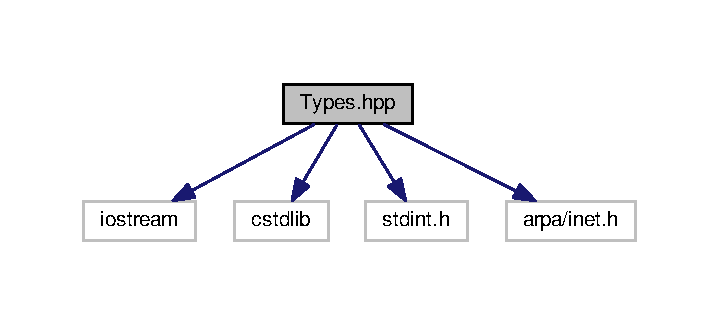
\includegraphics[width=345pt]{_types_8hpp__incl}
\end{center}
\end{figure}
This graph shows which files directly or indirectly include this file\-:\nopagebreak
\begin{figure}[H]
\begin{center}
\leavevmode
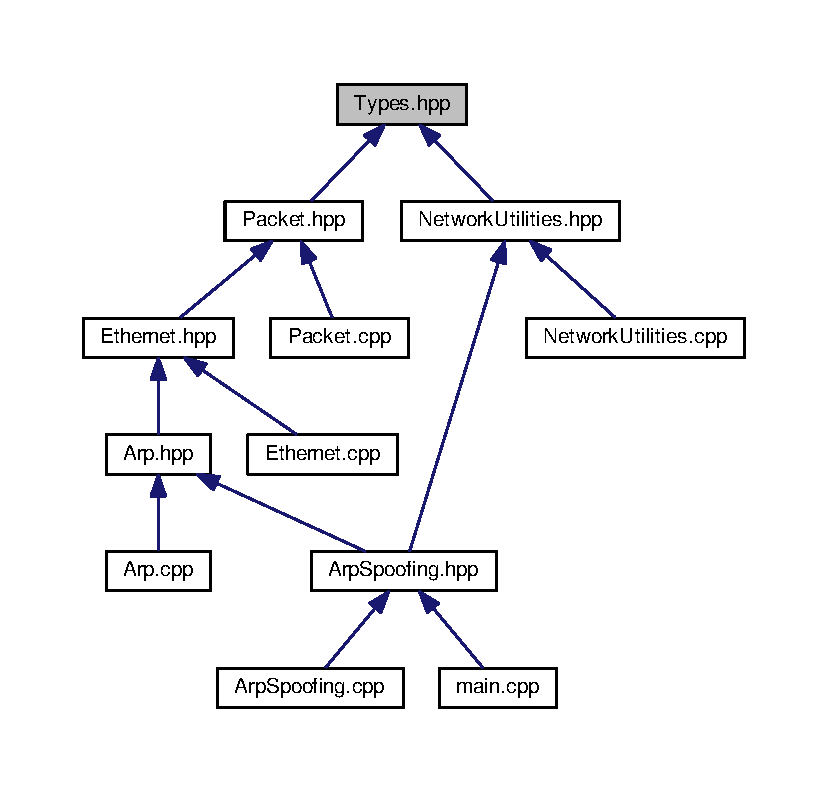
\includegraphics[width=350pt]{_types_8hpp__dep__incl}
\end{center}
\end{figure}
\subsection*{Classes}
\begin{DoxyCompactItemize}
\item 
struct \hyperlink{structuchar_mac}{uchar\-Mac}
\item 
struct \hyperlink{structuint8_ip}{uint8\-Ip}
\end{DoxyCompactItemize}
\subsection*{Typedefs}
\begin{DoxyCompactItemize}
\item 
\hypertarget{_types_8hpp_ab9abfa652ac5263df9eeeeb49d5f4691}{typedef struct \hyperlink{structuchar_mac}{uchar\-Mac} {\bfseries uchar\-Mac}}\label{_types_8hpp_ab9abfa652ac5263df9eeeeb49d5f4691}

\item 
\hypertarget{_types_8hpp_a7bbc832f6961fa55c4e6fa0ff3c88f59}{typedef struct \hyperlink{structuint8_ip}{uint8\-Ip} {\bfseries uint8\-Ip}}\label{_types_8hpp_a7bbc832f6961fa55c4e6fa0ff3c88f59}

\end{DoxyCompactItemize}


\subsection{Detailed Description}
Contains definitions of I\-P and M\-A\-C address. \begin{DoxyAuthor}{Author}
Jeremy Z\-Y\-R\-A 
\end{DoxyAuthor}
\begin{DoxyVersion}{Version}
1.\-0 
\end{DoxyVersion}

%--- End generated contents ---

% Index
\newpage
\phantomsection
\addcontentsline{toc}{chapter}{Index}
\printindex

\end{document}
